\chapter{Análisis}

	\noindent En este capítulo se presentará una breve descripción acerca del trabajo terminal haciendo mención del trabajo que se realizó, los problemas que se enfrentaron, así como lo que se logró. Continuando con el capítulo se presentan las Reglas de Negocio y las Reglas del Sistema donde se menciona que es lo que puede realizar la aplicación y que no.\\
	De manera breve  se hace mención de los casos de uso que se realizaron haciendo referencia al apartado Anexos para una consulta más detallada de cada uno de estos.\\
	Así mismo se menciona los Requisitos del usuario, Requisitos funcionales de la aplicación web y Requisitos no funcionales de la aplicación web.\\
	Finalmente se menciona las iteraciones programadas, detallando las actividades realizadas, problemas, logros y si fue necesario, investigación para lograr las metas propuestas.\\
	
	%Agregar etiqueta de diagrama de propuesto
	
	%=========================================================
	%                                                         Prototipo RIDESCOM
	%=========================================================
	\section{Prototipo para el Registro a Interpolit\'ecnicos Deportivos (RIDESCOM)}
	
	\noindent En este capítulo se muestran las iteraciones que realizamos los primeros 4 meses del año 2019 siguiendo la metodología Scrum. En las primeras iteraciones se realizó la investigación acerca de los aspectos fundamentales de las páginas web, con el finn de comprender los conceptos del desarrollo de aplicaciones y poder llevarlos a la práctica. En iteraciones posteriores se hizo un análisis de lo que va a realizar RIDESCOM; de ese análisis se obtuvieron los requisitos funcionales y no funcionales del sistema, una breve descripción de los casos de uso, así como la identificación de los actores, se fueron obteniendo reglas de negocio. Además, de seguir con la investigación y práctica de la creación de aplicaciones web y del uso o implementación de un crawler. Posteriormente se comenzó con la redacción de la documentación técnica, la investigación del estado del arte, el análisis y diseño de la base de datos, la comprensión de comandos de LaTeX, el diseño que tendrá la aplicación, se realizaron pantallas de como lucirá la apliación, se definieron los iconos que se utilizarán en la aplicación, se definieron las tecnologías a utilizar, se implementó un servidor local para la interacción con la aplicación móvil, se creó un primer prototipo de la aplicación con la vista del crawler (Inicio Sesión) y se realizó la redacción de este documento que es el reporte de actividades realizadas. También se creó el repositorio para el desarrollo colaborativo de los documentos. En estas iteraciones surgieron problemas e inconvenientes que afectan al proyecto RIDESCOM tales como la implementación de un crawler, la curva de aprendizaje del desarrollo utilizando Spring MVC, las limitaciones de tiempo debido a que los miembros del equipo trabajan o están realizando su servicio social. Pese a los problemas mencionados o no, tenemos un prototipo funcional de la aplicación así como la mayor parte de la documentación técnica y la elaboración de este documento. El resto de este capítulo presenta en mayor o menor medida los detalles del trabajo realizado en cada iteración.
	
	\section{An\'alisis de factibilidad t\'ecnica}
	
	%=========================================================
	%                                             Requisitos
	%=========================================================
	\section{Reglas de Negocio}
	\noindent La aplicación RIDESCOM permitirá a los alumnos que estén inscritos en el periodo actual, inscribirse en un evento interpolitécnico, consultar los eventos registrados, consultar calendario de eventos. 
	El sistema cuenta con una interfaz que nos permite visualizar las diferentes opciones ofrecidas por el mismo. Para acceder al anterior el usuario debe de tener un usuario y contraseña. Dicho usuario y contraseña, será con el que ingresa al sistema del SAES. 
	Así mismo, habrá “usuarios encargados”, quienes se encargan de controlar y supervisar el uso de éste ante pequeñas porciones de estudiantes (grupos de alumnos). Ahora dichos encargados hay dos tipos el Jefe de Fomento Deportivo, a este se le permitirá crear eventos deportivos, registrar eventos deportivos y restablecer contraseña a los perfiles de los coordinadores. El segundo tipo de encargado es el Coordinador de una Unidad Académica, este podrá registrar los resultados de los participantes en el sistema para poder ser visualizados en la vista principal, podrá generar un reporte de los alumnos registrados durante el periodo que se haya especificado y registrar a los entrenadores que laboran dentro de la Unidad Académica a la que atienda, a continuación se describirán las reglas para cada uno de los actores que se involucran.
	
	\subsection{Reglas de Negocio Jefe de Fomento Deportivo}
	Para que el JFD pueda ingresar a la página RIDESCOM debe de contar con un Usuario y Contraseña, de caso contrario no podrá acceder.
	Una vez dentro de la página de RIDESCOM se le mostrarán las opciones que tiene permitidas, tales como: Evento, Coordinadores, Usuarios, Pruebas en estos dos podrá agregar, editar o eliminar. \\
	
	\noindent Para la vista de Evento, la información se le mostrará en la página principal, si hay eventos registrados estos serán mostrados en la tabla correspondiente, sino se cuenta con datos se mostrará en la tabla el mensaje de que no existen datos.  Para poder agregar un evento se deben de cumplir con algunos campos que son requisito sino se completan los campos no podrá registrar el evento.  Dentro del formulario para crear el evento se debe asignar una fecha en la que los alumnos podrán inscribirse para esto, no debe de ser mayor  a 5 días en la que se realizará el evento. También se debe considerar que no se puede asignar una fecha menor respecto a la fecha en que se está creando el evento. Una vez tenga el evento registrado podrá editar información respecto a este, teniendo en cuenta los campos que son requisito, o en caso contrario eliminar el evento.\\
	
	\noindent Para la vista de Coordinadores, se mostrará la información en una tabla dentro de la página principal, en caso de no contar con datos registrados se mostrará un mensaje de que no existen datos. Para poder agregar un Coordinador de Unidad Académica deberá cumplir con campos que son requisitos sino se completan los campos no podrá registrar el coordinador. Una vez tenga el coordinador registrado podrá editar información respecto a este, teniendo en cuenta los campos que son requisito, o en caso contrario eliminar los datos del coordinador. \\
	
	\noindent Contará con un apartado en el que visualizará los resultados obtenidos por los participantes estos estarán disponibles hasta que concluyan los eventos interpolitécnios y para el JFD solo será de consulta. \\
	
	\noindent Para la vista de Pruebas, se mostrará una tabla en la que podrá ver las pruebas registradas, en caso de no tener datos que mostrar se mostrará un mensaje en el que se indique que no hay datos por mostrar. Se podrá agregar pruebas, para ello deberá de cumplir con los campos que son requisitos. De igual manera tendrá campos que son requisito para poder guardar los datos. Una vez guardado las Pruebas podrá editar o eliminar la información. \\
	\pagebreak
	
	\subsection{Reglas de Negocio Coordinador de Unidad Académica}
	\noindent Para que el Coordinador de Unidad Académica pueda ingresar a la página RIDESCOM debe de contar con un Usuario y Contraseña, de caso contrario no podrá acceder.\\
	
	\noindent Una vez dentro de la página de RIDESCOM se le mostrarán las opciones que tiene permitidas, tales como: Constancias, Calendario, Resultados, Consulta Inscritos, DIfundir Evento y Entrenadores. Las vistas antes mencionadas exceptuando Resultados y Difundir Evento, serán vistas de solo lectura.\\
	
	\noindent Para la vista de Constancias el Coordinador de la Unidad Académica podrá consultar si el alumno participó en un evento para que posteriormente, él pueda comenzar el trámite correspondiente para la generación de la constancia. Será solo vista de consulta/lectura.\\
	
	\noindent Para la vista de Calendario, se mostrará en la página principal del Coordinador una tabla con los datos que le corresponden, en caso de no tener información se mostrará el mensaje de que no existen datos. Esta vista sólo será de lectura.\\
	
	\noindent Para la vista de Resultados el Coordinador de la Unidad Académica podrá visualizar la información en una tabla dentro de la página principal, en caso de no tener datos se mostrará el mensaje de que no existen datos Para ingresar los resultados obtenidos de los participantes, como el tiempo que se obtuvo, el lugar, etc., deberá de llenar los campos que son requisitos, sino se completan los campos no podrá registrarse el evento. Una vez que se tengan los datos registrados podrá editar o eliminar estos.\\
	
	\noindent Para la vista Difundir Evento, el Coordinador de la Unidad Académica podrá visualizar los eventos que han sido registrados, al selecciona la opción difundir se le mostrará la opción de difundirlo en la red social de facebook.\\
	
	\noindent Para la vista de Entrenadores, se mostrará la información dentro de la vista principal en una tabla, en caso de no contar con información se mostrará el mensaje de que no existen datos. Para agregar datos de un Entrenador se deben de cumplir con datos que son requisitos. Una vez que se tengan datos registrados podrá editar o eliminar la información. \\
	
	\subsection{Reglas de Negocio Alumno}
	Para que el alumno pueda ingresar a la página RIDESCOM debe de contar con un Usuario y Contraseña, de caso contrario no podrá acceder.\\
	
	Una vez dentro de la página de RIDESCOM se le mostrarán las opciones que tiene permitidas, tales como: Calendario, Inscribe Interpolitecnico, Historial,  Resultados, Eventos Inscritos. Las vistas antes mencionadas serán solo lectura exeptuando la vista de INscribe Interpolitecnico.\\
	
	Para la vista de Calendario se mostrará en la página principal en una tabla que contenga la información, en caso de que esta no cuente con información se mostrará el mensaje de que no existen datos. Esta vista sólo será de lectura para el alumno.\\
	
	Para la vista de Inscribir Interpolitecnio, el alumno pueda inscribir un Evento Interpolitecnico deberá como primer punto, validar su status académico, para ello se le mostrará en segunda ocasión el inicio de sesión con esto, se verificará su estatus académico. Si el alumno está inscrito entonces se le mostrará una segundo vista en la que solo será de lectura y verificará si sus datos son correctos. En caso de que el alumno no esté inscrito se le mostrará un mensaje para notificarle que no puede inscribirse dado que no está inscrito en el periodo actual. \\
	Si la información que se le presenta es correcta podrá continuar para seleccionar el evento en el que desea participar y así concluir con su inscripción. \\
	
	Para la vista Historial, se mostrará al alumno una tabla que le proporcione información de los eventos en los que ha participado a lo largo de su trayectoria académica. Esta vista es de solo lectura.\\
	
	Para la vista Resultado, se mostrará la información de los resultados del último evento en el que a participado. Esta vista es de solo lectura.\\
	
	Para la vista de Eventos Inscritos, mostrará el o los eventos a los que se a registrado el alumno en el periodo en curso. Esta vista es de solo lectura.\\
	
	\noindent A continuación se mostrarán en distintas tablas las Reglas de Negocio de acuerdo a cada actor que involucra la aplicación.
	
	\begin{table}[hbt!]
		\begin{center}
			\begin{tabular}{|p{30mm}|p{100mm}|}
				\hline
				\multicolumn{2}{|c|}{Jefe de Fomento Deportivo} \\
				\hline
				Identificador & Descripción \\
				\hline 
				RN 1 & Para ingresar a la página debe de contar con un usuario y contraseña. \\ \hline
				RN 2 &  Para registrar un nuevo evento deben de completarse todos los campos que son requisito.\\ \hline
				RN 3 & Para registrar un evento debe de considerar que la fecha de este no sea menor a la fecha en la que se quiere realizar el mismo (no debe de ser mayor  a 5 días en la que se realizará el evento). \\ \hline
				RN 4 &  La fecha de inicio de registro para los alumnos no rebase la fecha en la que se realizará el evento.\\ \hline
				RN 5 &  La fecha de fin de registro para los alumnos no rebase la fecha en la que se realizará el evento. \\ \hline
				RN 6 & Para editar los datos de un evento, no debe de haber alumnos inscritos. \\ \hline
				RN 7 &  Al editar los datos de un evento debe considerar completar todos los campos.\\ \hline
				RN 8 &  Para eliminar un evento, no debe de haber alumnos inscritos en este.\\ \hline
				RN 9 &  Para agregar un deporte, todos los campos que son requisito deben completarse.\\ \hline
				RN 10 &  Al editar un deporte, se debe considerar completar todos los campos requeridos.\\ \hline
				RN 11 &  Para registrar una Prueba, se debe de completar todos los campos.\\ \hline
				RN 12 & Al editar los datos se debe considerar completar todos los campos.\\ \hline
				RN 13 &  Al registrar un nuevo Coordinador, se debe asignar un usuario y contraseña.\\ \hline
				RN 14 &  Para completar el registro, debe completarse todos los campos requeridos.\\ \hline
				RN 15 &  Al editar los datos de un Coordinador, se debe tomar en cuenta completar todos los campos requeridos.\\ \hline
				RN 16 &  Para registrar una Sede, deben completarse todos los campos requeridos.\\ \hline
				RN 17 &  Al editar los datos de una Sede, se debe considerar que esta no esté asignada en un evento.\\ \hline
			\end{tabular}
			\caption{Reglas de Negocio Jefe de Fomento Deportivo.}
			\label{RNJFD}
		\end{center}
	\end{table}
	
	\begin{table}[hbt!]
		\begin{center}
			\begin{tabular}{|p{30mm}|p{100mm}|}
				\hline
				\multicolumn{2}{|c|}{Coordinador de Unidad Acedémica} \\
				\hline
				Identificador & Descripción \\
				\hline 
				RN 18 &  Para ingresar a la página debe de contar con un usuario y contraseña.\\ \hline
				RN 19 & Las credenciales deben estar activas y ser proporcionadas por el Jefe de Fomento Deportivo.\\ \hline
				RN 20 & Para ingresar los resultados, debe seleccionar un usuario. \\ \hline
				RN 21 & Se debe seleccionar una prueba correspondiente al alumno.\\ \hline
				RN 22 & Para terminar el proceso de registro de resultados, debe completar los campos requeridos. \\ \hline
				RN 23 & Para registrar un entrenador debe llenar todos los campos requeridos.\\ \hline
				RN 24 & Para obtener la cédula de inscripción, el coordinador deberá de seleccionar el tipo de deporte, así como el ciclo escolar. \\ \hline
				RN 25 & Para consultar si un alumno participó en un evento, se debe buscar por medio de su boleta o por el ciclo escolar en el que participó.\\ \hline
				RN 26 & Para difundir un evento, deberá seleccionar el evento de la tabla y seleccionar el medio por el cual quiere compartir el evento.\\ \hline
			\end{tabular}
			\caption{Reglas de Negocio Coordinador de Unidad Académicas.}
			\label{RNCUA}
		\end{center}
	\end{table}
	
	\pagebreak
	
	\begin{table}[hbt!]
		\begin{center}
			\begin{tabular}{|p{30mm}|p{100mm}|}
				\hline
				\multicolumn{2}{|c|}{Alumno} \\ \hline
				Identificador & Descripción \\ \hline 
				RN & Para ingresar a la página debe de contar con un usuario y contraseña.\\ \hline
				RN & El alumno debe verificar el estatus académico para poder registrarse en un evento.\\ \hline
				RN & Para concluir el registro al evento, debe de llenar todos los campos requeridos.\\ \hline
				RN & Puede inscribirse en los eventos que desee, siempre y cuando no tenga traslape en horas de los eventos.\\ \hline
				RN & \\ \hline
				RN & \\ \hline
			\end{tabular}
			\caption{Reglas de Negocio para el alumno.}
			\label{RNA}
		\end{center}
	\end{table}
	
	
	%=========================================================
	%                                             Requisitos
	%=========================================================
	\section{Reglas del Sistema}
	\noindent El alumno que desee participar en un evento interpolitécnico hará uso de la aplicación web RIDESCOM. Como primer punto deberá iniciar sesión en la misma, ingresando el usuario y contraseña con el que entra a sistema SAES (Sistema de Administración Escolar). Si los datos ingresados son correctos, se le dará acceso a la aplicación RIDESCOM, en caso contrario no se le dará acceso para poder registrarse en un evento. Sin embargo, podrá seguir visualizando datos generales, como lo es el calendario de eventos, resultados de eventos y los eventos que se practican dentro de la unidad académica.
	El Jefe de Fomento Deportivo podrá dar de alta a un Coordinador de alguna Unidad Académica. Para dar de alta un evento deportivo deberá llenar todos los campos requeridos, tendrá la opción de agregar una descripción si así lo desea. 
	El Coordinador de la Unidad Académica registrará a los entrenadores de las actividades deportivas deberá llenar los campos requeridos para poder concluir el registro. En caso de que exista un entrenador ya haya sido registrado, la aplicación le notificará. Una vez concluido los eventos deportivos, este registrará los resultados obtenidos por los participantes para que puedan ser vistos por la comunidad en general. \pagebreak
	
	
	%=========================================================
	%                                    Diagrama de procesos
	%=========================================================
	\section{Diagrama de Procesos}
		\noindent En este apartado se explicará y detallará el proceso actual que sigue el alumno para poder registrarse en un evento interpolitécnico deportivo, posteriormente se hace mención del proceso porpuesto para el mismo fin.\\
		El proceso actual que el alumno debe seguir para inscribirse a un evento interpolitécnico deportivo comienza cuando el alumno acude al Deportamento de Actividades Deportivas de su unidad académica donde el encargado del departamento le proporciona un formato el cual debe llenar a mano. Este formato se debe de llenar de acuerdo al número de eventos en el que el alumno quiera participar.\\
		El formato antes mencionado solicita campos como: nombre, deporte, escuela, prueba, entre otros. Una vez completado el formato el alumno entrega su solicitud al encargado del Departamento y este hace mención que se comunicarán con el en cuanto se tenga una actualización acerca de su solicitud.\\
		\noindent El proceso continua con el encargado del Departamento de Actividades Deportivas quien genera una lista de alumnos solicitantes para posteriormente comprobar su estatus académico. Esto se realiza ya que según el reglamento solo los alumnos participantes son los que pueden participar en los eventos.
		Una vez que realizada la comprobación se le notifica al alumno el estatus final de su solicitud, sea aceptada o rechazada.
		El coordinador de la unidad académica realiza un listado con los alumnos que participaran en los eventos de acuerdo al ciclo escolar en curso para que sea enviado al Departamento de Fomento Deportivo.
		Finalmente el alumno espera a que sea la fecha del evento para hacer su participación. Una vez concluido estos, se procede a pagar el arbitraje que se contrata para llevar control de las actividades deportivas.\\
		\noindent Una vez pagado el arbitraje se pasa a hacer el llenado de los resultados obtenidos para cada uno de los participantes para así ser publicados y pueda ser visualizados por la comunidad estudiantil.
	
	
	%=========================================================
	%                                            Casos de Uso
	%=========================================================
	\section{Casos de Uso}
	En esta sección se describe cada uno de los procesos que se debe de tener la aplicación web tomando en cuenta las reglas de negocio, los requisitos funcionales y los requisitos no funcionales, así como la problemática que ataca el proyecto.
%		\subsection{CU1 Iniciar Sesión Jefe de Fomento Deportivo}
%		\noindent En este caso de uso describe el funcionamiento del módulo Iniciar sesión para el Jefe de Fomento Deportivo. Se describe paso a paso el proceso a seguir, asi como los posibles errores que pueden existir junto con los mensajes correspondientes para cada caso. Para mas detalles consulta el apartado Anexos en la sección \ref{CasosdeUso} haciendo referencia al CU \ref{CU1_Iniciarsesion}. \\
		\begin{UseCase}{CU1}{Iniciar Sesión Jefe de Fomento Deportivo}{
		\noindent Esta caso de uso servirá para que el Jefe de Fomento Deportivo pueda ingresar a la página web, poder identificar al usuario y así mostrar las vistas que tienen asginada. \\
    	Para poder iniciar sesión el actor deberá oprimir el botón \IUbutton{ Iniciar Sesión } ubicado en la pantalla \ref{inicioJFDycoord}. Ingresará su número de boleta, contraseña el cual usa para ingresar al SAES (Sistema de Administración Escolar), y el captcha, como se muestra en la pantalla... Si los datos que ingresa no coinciden se le mostrará un mensaje.
        Una vez que incie sesión se le mostrará la pantalla principal.
        \MSGref{MSG1}{Campos requeridos}.
        
	} \label{CU1_Iniciarsesion}
		\UCitem{Versión}{0.1}
		\UCitem{Autor}{Rosales González Carlos Andrés}
		\UCitem{Supervisa}{Mendoza García Bruno Alejandro}
		\UCitem{Actor}{Jefe de Fomento Deportivo}
		\UCitem{Propósito}{Tener control de las personas registradas.}
        \UCitem{Precondiciones}{
        \begin{itemize}
            \item Contar con una cuenta.
            \item Contar con la contraseña.
        \end{itemize}}
        \UCitem{Postcondiciones}{Se muestra la pantalla principal}
		\UCitem{Entradas}{
        \begin{itemize}
        	\item Usuario. 
        	\item Contraseña
        \end{itemize}}
		\UCitem{Origen}{Pantalla, Teclado}
		\UCitem{Salidas}{
		\begin{itemize}
		    \item Acceso a la página principal del Jefe de Fomento Deportivo
		\end{itemize}}
		\UCitem{Destino}{Pantalla}
		\UCitem{Errores}{
        	\begin{itemize}
        	    \item Los campos están vacíos.
            	\item Usuario y/o contraseña incorrecta.
            \end{itemize}
       }
		\UCitem{Observaciones}{}
		\end{UseCase}
	\newpage
	
    \begin{UCtrayectoria}{Principal}
    \UCpaso[\UCactor] Ingresa a la página RIDESCOM.
    \UCpaso Muestra la pantalla \IUref{}{Pantalla de Inicio de Sesión \ref{inicioJFDycoord}}.
    \UCpaso[\UCactor] Oprime el botón \IUbutton{ JFD o Coordinador } que esta en la \IUref{}{Pantalla de Inicio de Sesión \ref{inicioJFDycoord}}.
    \UCpaso Muestra la \IUref{}{Pantalla de Inicio de Sesión \ref{inicioJFDycoord}}
	\UCpaso[\UCactor] Introduce Usuario y contraseña. \label{CU1_regresar} 
    \UCpaso[\UCactor] Presiona el botón \IUbutton{ Ingresar }.
    \UCpaso Comprueba que los campos no estén vacíos. \Trayref{A}
    \UCpaso Obtiene los valores ingresados
    \UCpaso Válida campos. \Trayref{B}
    \UCpaso Muestra la \IUref{}{Pantalla principal del Jefe de Fomento Deportivo. \ref{principalJFD}}
    \end{UCtrayectoria}
    
    \begin{UCtrayectoriaA}{A}{Campo(s) vacios}
    	\UCpaso muestra mensaje “CamposNecesario".
    	\UCpaso Continua en el paso \ref{CU1_regresar} del \UCref{CU1}.
    \end{UCtrayectoriaA}

	\begin{UCtrayectoriaA}{B}{Boleta y/o contraseña erróneo}
		\UCpaso muestra mensaje “El usuario y/o contraseña que se ingresó son erróneos”. Mensaje .
   		\UCpaso Continua en el paso \ref{CU1_regresar} del \UCref{CU1}.
	\end{UCtrayectoriaA}

	



		
%		\subsection{CU2 Iniciar Sesión Coordinador de Unidad Académica}
%		\noindent En este caso de uso describe el funcionamiento del módulo Iniciar sesión para el Coordinador de Unidad Académica. Se describe paso a paso el proceso a seguir, asi como los posibles errores que pueden existir junto con los mensajes correspondientes para cada caso. Para mas detalles consulta el apartado Anexos en la sección \ref{CasosdeUso} haciendo referencia al CU \ref{CU2_Iniciarsesion}. \\
		\begin{UseCase}{CU1.1}{Inicio Sesión}{
		Servirá para que el alumno pueda ingresar a la aplicación y así poder inscribirse en algún evento de su interés o consultar los eventos a los que ya se ha registrado previamente. \\
        En caso de que el alumno ingrese una boleta la cual no a sido registrada, se mostrará un mensaje el cual le indique que la boleta que ingreso no existe. Mensaje . De igual manera, si la contraseña es diferente a la que se registro aparecerá un mensaje que le indique que la contraseña no coincide. Mensaje .
	}
		\UCitem{Versión}{0.1}
		\UCitem{Autor}{Rosales González Carlos Andrés}
		\UCitem{Supervisa}{Mendoza García Bruno Alejandro}
		\UCitem{Actor}{Alumno}
		\UCitem{Propósito}{Tener control de las personas registradas.}
        \UCitem{Precondiciones}{
        \begin{itemize}
            \item Haberse registrado
            \item Perfil valido por el coordinador
        \end{itemize}}
        \UCitem{Postcondiciones}{Ninguna}
		\UCitem{Entradas}{
        \begin{itemize}
        	\item Número de boleta 
        	\item Contraseña
        \end{itemize}}
		\UCitem{Origen}{Pantalla, Teclado}
		\UCitem{Salidas}{
		\begin{itemize}
		    \item Acceso a la página principal del alumno
		\end{itemize}}
		\UCitem{Destino}{Pantalla}
		\UCitem{Errores}{
        	\begin{itemize}
        	    \item Los campos están vacíos.
            	\item No existe la boleta. Mensaje .
            	\item Contraseña incorrecta. Mensaje .
            \end{itemize}
       }
		\UCitem{Observaciones}{}
		\end{UseCase}
    \begin{UCtrayectoria}{Principal}
    \UCpaso[\UCactor] Oprime el botón Iniciar Sesión en la pantalla.
    \UCpaso Muestra la pantalla.
	\UCpaso[\UCactor] Introduce Boleta y contraseña. 
    \UCpaso[\UCactor] Presiona el botón Ingresar.
    \UCpaso Comprueba que los campos no estén vacíos. \Trayref{A} \Trayref{B} \Trayref{C}
    \UCpaso Obtiene los valores ingresados
    \UCpaso Válida campos. 
    \UCpaso Muestra la pantalla .
    \end{UCtrayectoria}
    
	\begin{UCtrayectoriaA}{A}{No hay dato insertado en el campo solicitado}
		\UCpaso muestra mensaje “Error: Los campos están vacíos por favor asegúrese de poner lo que se pide”. Mensaje .
		\UCpaso Regresa al paso 3 de la Trayectoria Principal.
	\end{UCtrayectoriaA}
	
	\begin{UCtrayectoriaA}{B}{}
		\UCpaso muestra mensaje “No existe boleta ingresada”. Mensaje .
		\UCpaso Regresa al paso 2 de la trayectoria principal.
	\end{UCtrayectoriaA}
	
	\begin{UCtrayectoriaA}{C}{}
		\UCpaso muestra mensaje “Contraseña incorrecta”. Mensaje .
		\UCpaso Regresa al paso 2 de la trayectoria principal.
	\end{UCtrayectoriaA}
		
%		\subsection{CU3 Iniciar Sesión Alumno}
%		\noindent En este caso de uso describe el funcionamiento del módulo Iniciar sesión para el Alumno. Se describe paso a paso el proceso a seguir, asi como los posibles errores que pueden existir junto con los mensajes correspondientes para cada caso. Para mas detalles consulta el apartado Anexos en la sección \ref{CasosdeUso} haciendo referencia al CU \ref{CU3_Iniciarsesion}.\\
		\begin{UseCase}{CU3}{Inscribir a un evento interpolitécnico deportivo}{
		\noindent Este caso de uso permite que el actor alumno, pueda registrarse en el evento interpolitécnico deportivo de su interés. Deberá llenar un formulario donde se solicitan datos del alumno como: Grupo, NSS (Número de Seguro Social), correo electrónico, Delegación/Municipio, así como el seleccionar el deporte en el que desea participar.\\
        Para poder inscribirse, deberá primero validar su estatus académico (Inscrito/No inscrito), para ello debe ingresar su boleta, contraseña y el captcha como se muestra en la pantalla \IUref{p15InscripcionInterpolitecnico1}{Pantalla Inscribir interpolitécnico 1.}, da click en el botón \IUbutton { Verificar } si cumple con el requisito, continua el proceso, en caso contrario no podrá inscribirse en algun evento interpolitécnico deportivo.\\
        El siguiente paso es la verificación de datos como se muestra en la pantalla \IUref{p15InscripcionInterpolitecnico2}{Pantalla Inscribir interpolitécnico 2.}, si los datos son correctos da click en el botón \IUbutton{ Aceptar }\\
        Si los datos son correctos, da click en el botón \IUbutton{ Aceptar }, a continuación se muestra la pantalla \IUref{p15InscripcionInterpolitecnico3}{Pantalla Inscribir interpolitécnico 3.} donde llenará los datos corresponidentes al evento deportivo. Una vez que se llenen todos los campos, el alumno da click en el botón \IUbutton{ Inscribir }.\\ 
        Al final se mostrará un mensaje de confirmación de la inscripción.
	}
		\UCitem{Versión}{0.1}
		\UCitem{Autor}{Rosales González Carlos Andrés}
		\UCitem{Supervisa}{Mendoza García Bruno Alejandro}
		\UCitem{Actor}{Alumno}
		\UCitem{Propósito}{Poder participar en un evento deportivo.}
        \UCitem{Precondiciones}{
        \begin{itemize}
            \item Iniciar Sesión
            \item Ser un alumno pertenenciente al IPN
            \item Validar estatus académico
        \end{itemize}}
        \UCitem{Postcondiciones}{Persitencia de dat}
		\UCitem{Entradas}{
        \begin{itemize}
        	\item Boleta, contraseña y captcha
        	\item Grupo, Escuela, Carrera
        	\item Nombre, Apellido, Sexo
        	\item Curp, Fecha de nacimiento, Lugar
        	\item NSS, Correo electrónico, Delegación
        	\item Deporte, Sub-division, Prueba, Fecha del evento
        \end{itemize}}
		\UCitem{Origen}{Teclado}
		\UCitem{Salidas}{
		\begin{itemize}
		    \item Confirmación de la inscripción al evento
		\end{itemize}}
		\UCitem{Destino}{Pantalla principal}
		\UCitem{Errores}{
        	\begin{itemize}
            	\item EL alumno no se encuentra inscrito en el periodo actual.
            	\item Completa todos los campos
            \end{itemize}
       }
		\UCitem{Observaciones}{}
		\end{UseCase}
    \begin{UCtrayectoria}{Principal}
    \UCpaso[\UCactor] Oprime el botón \IUbutton { Inscribir Interpolitécnico } de la pantalla \IUref{p13Iniciopaticipante}{Pantalla principal del alumno \ref{Inscripcioninterpolitecnico}}.\label{CU3_inicio}
    \UCpaso Muestra la pantalla \IUref{p15InscripcionInterpolitecnico1}{Pantalla Inscribir interpolitécnico 1 \ref{Inscripcioninterpolitecnico2}.}\label{CU3_regresa}
    \UCpaso[\UCactor] Ingresa boleta, contraseña y captcha.
    \UCpaso[\UCactor] Da click en el botón \IUbutton { Verificar }
    \UCpaso Envia los datos mediante el crawler a la página del SAES.
    \UCpaso Verifica si hay acceso al SAES. \Trayref{A} \Trayref{B}
    \UCpaso Muestra la pantalla \IUref{p15InscripcionInterpolitecnico2}{Pantalla Inscribir interpolitécnico 2 \ref{Inscripcioninterpolitecnico3}}.
    \UCpaso Muestra los datos personales del alumno.
	\UCpaso[\UCactor] Da click en el botón \IUbutton {Aceptar}. \Trayref{C}
	\UCpaso Busca los deportes y subdivisiones asociados a la unidad académica del alumno que esta haciendo la solicitud.
	\UCpaso Muestra la pantalla \IUref{p15InscripcionInterpolitecnico3}{Pantalla Inscribir interpolitécnico 3.}. \label{CU3_deporte}
	\UCpaso[\UCactor] Llena los campos solicitados. \Trayref{D}
    \UCpaso Confirma registro en una ventana emergente.
    \UCpaso Carga la pantalla Principal.
    \end{UCtrayectoria}
    
	\begin{UCtrayectoriaA}{A}{El alumno debe de estar inscrito para continuar.}
		\UCpaso Muestra el mensaje. “El alumno no esta inscrito en el periodo actual”
   		\UCpaso Continua en el paso \ref{CU3_regresa} del \UCref{CU3}.
	\end{UCtrayectoriaA}
	
	\begin{UCtrayectoriaA}{B}{El alumno cancela el proceso de Inscribir interpolitécnico}
		\UCpaso[\UCactor] Da click en el botón \IUbutton { Cancelar } de la pantalla \IUref{p15InscripcionInterpolitecnico1}{Pantalla Inscribir interpolitécnico 1.}
		\UCpaso  Continua en el paso \ref{CU3_inicio} del \UCref{CU3}.
	\end{UCtrayectoriaA}

	\begin{UCtrayectoriaA}{C}{Los datos del alumno no coinciden}
		\UCpaso[\UCactor] Da click en el botón \IUbutton { Cancelar } de la pantalla \IUref{p15InscripcionInterpolitecnico2}{Pantalla Inscribir interpolitécnico 2.}
		\UCpaso Continua en el paso \ref{CU3_inicio} del \UCref{CU3}.
	\end{UCtrayectoriaA}
	
	\begin{UCtrayectoriaA}{D}{El alumno no completa los campos requeridos}
		\UCpaso Muestra el mensaje "Debes llenar todos los campos solicitados". \ref{CU3_deporte}
		\UCpaso Continua en el paso \ref{CU3_inicio} del \UCref{CU3}.
	\end{UCtrayectoriaA}
		
%		\subsection{CU4 Recuperar contraseña para el alumno}
%		\noindent Este caso de uso se define para que el alumno pueda recuperar la contraseña, sin embargo dado que el alumno ingresa a la aplicación web con el usuario y contraseña que utiliza al accesar al SAES, será re dirigido a la antes mencionada para que solicite su nueva contraseña. Para más detalles consulte el apartado Anexos en la sección \ref{CasosdeUso} haciendo referencia al CU \ref{CU4_Recuperaalum}. \\ \pagebreak
		\begin{UseCase}{CU}{Registro}{
		Servirá para que el alumno que esté interesado en participar en algún evento interpolitécnico deportivo, cree una cuenta para posteriormente poder iniciar sesión y así, inscribirse en el evento de su interés. 
		Dicho registro lo encontrará dentro de la pantalla de Inicio en el apartado ‘Regístrate’, posteriormente deberá llenar los campos que se le solicitan, los cuales son: Boleta, Correo electrónico y una contraseña.
		El numero de Boleta consta de 10 caracteres numéricos, y en el correo solamente se aceptan los dominios más comunes (Gmail, Hotmail, Outlook).
		Una vez realizado, el alumno deberá acudir al Departamento de Actividades Deportivas de su Unidad Académica en un periodo no máximo a los 3 días a partir del día en el que se registró, para que el coordinador valide los datos que se ingresaron previamente. Para ello el coordinador deberá solicitar una identificación escolar vigente para corroborar dichos datos. }
		\label{CU_Registro}
	
	\UCitem{Versión}{0.1}
	\UCitem{Autor}{Rosales González Carlos Andrés}
	\UCitem{Supervisa}{Mendoza García Bruno Alejandro}
	\UCitem{Actor}{Alumno}
	\UCitem{Propósito}{Poder inscribirse en un evento interpolitécnico deportivo.}
	\UCitem{Precondiciones}{No estar registrado previamente}
	\UCitem{Postcondiciones}{
		\begin{itemize}
			\item El alumno podrá ingresar al sistema.
			\item Habrá un registro nuevo del alumno.
			\item Deberá acudir en un periodo no máximo a 3 días al Departamento de Actividades Deportivas de su Unidad Académica.
	\end{itemize}}
	\UCitem{Entradas}{
		\begin{itemize}
			\item Número de boleta 
			\item Contraseña
			\item Correo electrónico
	\end{itemize}}
	\UCitem{Origen}{Pantalla, Teclado}
	\UCitem{Salidas}{Pantalla}
	\UCitem{Destino}{Pantalla principal}
	\UCitem{Errores}{
		\begin{itemize}
			\item La boleta no es válida
			\item Dominio de correo invalido
		\end{itemize}
	}
	\UCitem{Observaciones}{Ninguna}
\end{UseCase}
\begin{UCtrayectoria}{Principal}
	\UCpaso[\UCactor] Oprime el \IUbutton{ Registrate  } ubicado en la pantalla Principal.
	%\UCpaso Muestra el mensaje {\bf MSG1-}``¿Está [{\em seguro}] de querer eliminar este registro.''.
	\UCpaso Se conecta al SAES y obtiene el CAPTCHA del login.
	\UCpaso Muestra la pantalla.
	\UCpaso[\UCactor] Introduce Boleta, Contraseña y correo electronico
	\UCpaso[\UCactor] Presiona el botón.
	\UCpaso Comprueba los campos obligatorios que no estén vacias.
	\UCpaso Inicia sesión en el SAES de la escuela usando la boleta, contraseña y captcha introducidos.
	\UCpaso verifica que el alumno está efectivamente inscrito \Trayref{A} \Trayref{B}
	\UCpaso Registra al alumno.
	\UCpaso Muestra el mensaje MSG1 “Registro de cuenta exitoso”.
	\UCpaso Muestra la pantalla .
\end{UCtrayectoria}

\begin{UCtrayectoriaA}{A}{Inserta algún otro carácter no correspondiente al “Número de Boleta” y presiona el botón ‘Registrar’}
	\UCpaso Muestra en la ventana el mensaje “Número de Boleta inválido”
	\UCpaso Regresa al paso 2 de la trayectoria principal.
\end{UCtrayectoriaA}

\begin{UCtrayectoriaA}{B}{Inserta algún otro carácter no correspondiente al “Dominio del correo electrónico” y presiona el botón ‘Registrar’}
	\UCpaso Muestra en la ventana el mensaje “Correo inválido, asegúrese que su correo sea de tipo Gmail, Hotmail o Outlook”
	\UCpaso Regresa al paso 2 de la trayectoria principal.
\end{UCtrayectoriaA}

		
%		\subsection{CU5 Recuperar contraseña para el coordinador}
%		\noindent Este caso de uso sirve para que el coordinador de unidad académica solicite el restablecer la contraseña. Sin embargo, para que esta sea restablecida el coordinador debe solicitarla mediante un oficio o escrito para que se tenga la certeza de que este es quien realmente hace la solicitud. Para más detalles consulte el apartado Anexos en la sección \ref{CasosdeUso} haciendo referencia al CU \ref{CU5_Recupercoord}.\\ 
		\begin{UseCase}{CU}{Validación de perfil}{
		Servirá para que el alumno que esté interesado en participar en algún evento interpolitécnico deportivo, cree una cuenta para posteriormente poder iniciar sesión y así, inscribirse en el evento de su interés. 
		Dicho registro lo encontrará dentro de la pantalla de Inicio en el apartado ‘Regístrate’, posteriormente deberá llenar los campos que se le solicitan, los cuales son: Boleta, Correo electrónico y una contraseña.
		El numero de Boleta consta de 10 caracteres numéricos, y en el correo solamente se aceptan los dominios más comunes (Gmail, Hotmail, Outlook).
		Una vez realizado, el alumno deberá acudir al Departamento de Actividades Deportivas de su Unidad Académica en un periodo no máximo a los 3 días a partir del día en el que se registró, para que el coordinador valide los datos que se ingresaron previamente. Para ello el coordinador deberá solicitar una identificación escolar vigente para corroborar dichos datos. }
		\label{CU_Validacionperfil}
	
	\UCitem{Versión}{0.1}
	\UCitem{Autor}{Rosales González Carlos Andrés}
	\UCitem{Supervisa}{Mendoza García Bruno Alejandro}
	\UCitem{Actor}{Alumno}
	\UCitem{Propósito}{Poder inscribirse en un evento interpolitécnico deportivo.}
	\UCitem{Precondiciones}{No estar registrado previamente}
	\UCitem{Postcondiciones}{
		\begin{itemize}
			\item El alumno podrá ingresar al sistema.
			\item Habrá un registro nuevo del alumno.
			\item Deberá acudir en un periodo no máximo a 3 días al Departamento de Actividades Deportivas de su Unidad Académica.
	\end{itemize}}
	\UCitem{Entradas}{
		\begin{itemize}
			\item Número de boleta 
			\item Contraseña
			\item Correo electrónico
	\end{itemize}}
	\UCitem{Origen}{Pantalla, Teclado}
	\UCitem{Salidas}{Pantalla}
	\UCitem{Destino}{Pantalla principal}
	\UCitem{Errores}{
		\begin{itemize}
			\item La boleta no es válida
			\item Dominio de correo invalido
		\end{itemize}
	}
	\UCitem{Observaciones}{Ninguna}
\end{UseCase}
\begin{UCtrayectoria}{Principal}
	\UCpaso[\UCactor] Oprime el \IUbutton{ Registrate  } ubicado en la pantalla Principal.
	%\UCpaso Muestra el mensaje {\bf MSG1-}``¿Está [{\em seguro}] de querer eliminar este registro.''.
	\UCpaso Se conecta al SAES y obtiene el CAPTCHA del login.
	\UCpaso Muestra la pantalla.
	\UCpaso[\UCactor] Introduce Boleta, Contraseña y correo electronico
	\UCpaso[\UCactor] Presiona el botón.
	\UCpaso Comprueba los campos obligatorios que no estén vacias.
	\UCpaso Inicia sesión en el SAES de la escuela usando la boleta, contraseña y captcha introducidos.
	\UCpaso verifica que el alumno está efectivamente inscrito \Trayref{A} \Trayref{B}
	\UCpaso Registra al alumno.
	\UCpaso Muestra el mensaje MSG1 “Registro de cuenta exitoso”.
	\UCpaso Muestra la pantalla .
\end{UCtrayectoria}

\begin{UCtrayectoriaA}{A}{Inserta algún otro carácter no correspondiente al “Número de Boleta” y presiona el botón ‘Registrar’}
	\UCpaso Muestra en la ventana el mensaje “Número de Boleta inválido”
	\UCpaso Regresa al paso 2 de la trayectoria principal.
\end{UCtrayectoriaA}

\begin{UCtrayectoriaA}{B}{Inserta algún otro carácter no correspondiente al “Dominio del correo electrónico” y presiona el botón ‘Registrar’}
	\UCpaso Muestra en la ventana el mensaje “Correo inválido, asegúrese que su correo sea de tipo Gmail, Hotmail o Outlook”
	\UCpaso Regresa al paso 2 de la trayectoria principal.
\end{UCtrayectoriaA}
		
%		\subsection{CU6 Consulta calendario de eventos}
%		\noindent Este caso de uso tiene como finalidad el mostrar a los usuarios dentro de la aplicación web, los eventos interpolitécnicos deportivos disponibles para registrase. Para más detalles consulte el apartado Anexos en la sección \ref{CasosdeUso} haciendo referencia al CU \ref{CU6_evento}. \\
		\begin{UseCase}{CU6}{Consulta Calendario de Eventos}{
		\noindent Este caso de uso tiene como finalidad mostrar la las fechas en la que los eventos registrados se van a realizar, el actor pueda consultar en la página principal los eventos que han sido registrados y están disponibles para inscribirse. 
		Para ello deberá iniciar sesión, una vez hecho esto se mostrará una pantalla  donde estarán las opciones que este tenga disponibles y a su vez, el calendario de eventos estará contenida en esta misma como se puede apreciar en \IUref{}{Pantalla de Principal \ref{principalalum}}.
        
	} \label{CU6_evento}
		\UCitem{Versión}{0.1}
		\UCitem{Autor}{Rosales González Carlos Andrés}
		\UCitem{Supervisa}{Mendoza García Bruno Alejandro}
		\UCitem{Actor}{Jefe de Fomento Deportivo, Coordinador de Unidad Académica, Alumno}
		\UCitem{Propósito}{Consultar los eventos disponibles.}
        \UCitem{Precondiciones}{
        \begin{itemize}
            \item Iniciar sesión.
        \end{itemize}}
        \UCitem{Postcondiciones}{Se muestra la pantalla principal}
		\UCitem{Entradas}{
        \begin{itemize}
        	\item Nombre Eventos
        	\item Deporte
        	\item Fecha del Evento
        	\item Descripcion
    	    \item Ciclo escolar
        \end{itemize}}
		\UCitem{Origen}{Pantalla, Teclado}
		\UCitem{Salidas}{
		\begin{itemize}
		    \item Eventos registrados
		\end{itemize}}
		\UCitem{Destino}{Pantalla Principal}
		\UCitem{Errores}{
        	\begin{itemize}
        	    \item No hay eventos registrados.
            \end{itemize}
       }
		\UCitem{Observaciones}{}
		\end{UseCase}
	\pagebreak
	
    \begin{UCtrayectoria}{Principal}
    \UCpaso[\UCactor] Ingresa a la página RIDESCOM.
    \UCpaso Muestra la pantalla \IUref{}{Pantalla de Inicio de Sesión \ref{principalalum}}.
    \UCpaso Muestra los eventos registrados.  \Trayref{A} \label{CU6_regresar}
    \UCpaso[\UCactor] Se desplaza dentro de la \IUref{}{Pantalla de Principal \ref{principalJFD}} para visualizar todos los campos registrados.
	\UCpaso[\UCactor] Consulta los eventos. 
    \end{UCtrayectoria}

	\begin{UCtrayectoriaA}{A}{No existen registros}
		\UCpaso Muestra mensaje “No existen registros.".
		\UCpaso Continua en el paso \ref{CU6_regresar} del \UCref{CU6}.
	\end{UCtrayectoriaA}
    

	



		
%		\subsection{CU7 Alta de eventos deportivos}
%		\noindent Este caso de uso tiene como finalidad el agregar un nuevo evento deportivo, solicitando los datos indispensables para que sea de fácil entender y ubicación. Para más detalles consulte el apartado Anexos en la sección \ref{CasosdeUso} haciendo referencia al CU \ref{CU7_evento}.\\
		\begin{UseCase}{CU7}{Alta de Eventos Deportivos}{
		\noindent Este caso de uso servirá para que el Jefe de Fomento Deportivo pueda ingresar a la página web los eventos que estarán disponibles durante el ciclo escolar en curso y así pueda ser visualizado por la comunidad y quién quiera participar en un evento pueda consultar los datos relevantes de este.
		Para ello el Jefe de Fomento Deportivo dará click en el botón \IUbutton{ + Agregar Evento } ubicado en la  parte superior de la tabla de calendario dentro de la \IUref{}{Pantalla de Inicio de Sesión \ref{principalJFD}}.	
	} \label{CU7_evento}

		\UCitem{Versión}{0.1}
		\UCitem{Autor}{Rosales González Carlos Andrés}
		\UCitem{Supervisa}{Mendoza García Bruno Alejandro}
		\UCitem{Actor}{Jefe de Fomento Deportivo}
		\UCitem{Propósito}{Registrar eventos Interpolitécnicos Deportivos.}
        \UCitem{Precondiciones}{
        \begin{itemize}
            \item Iniciar sesión.
        \end{itemize}}
        \UCitem{Postcondiciones}{Se muestra la pantalla principal}
		\UCitem{Entradas}{
        \begin{itemize}
        	\item Nombre del evento 
        	\item Dirección
        	\item Sede
        	\item Punto de Referencia
        	\item Semestre
        	\item Fecha inicio de registro
        	\item Fecha fin de registro
        	\item Deporte
        	\item Comentarios
        \end{itemize}}
		\UCitem{Origen}{Pantalla, Teclado}
		\UCitem{Salidas}{
		\begin{itemize}
		    \item Evento registrado
		    \item Campos requeridos
		\end{itemize}}
		\UCitem{Destino}{Pantalla}
		\UCitem{Errores}{
        	\begin{itemize}
        	    \item Los campos están vacíos..
            \end{itemize}
       }
		\UCitem{Observaciones}{}
		\end{UseCase}
	
    \begin{UCtrayectoria}{Principal}
    \UCpaso[\UCactor] Ingresa a la \IUref{}{Pantalla Registrar un Evento Interpolitécnico Deportivo \ref{creaevento}}.
    \UCpaso Muestra la \IUref{}{Pantalla Registrar un Evento Interpolitécnico Deportivo \ref{creaevento}}.
    \UCpaso[\UCactor] Llena los campos solicitados. \label{CU7_regresar}
    \UCpaso[\UCactor] Presiona el botón \IUbutton{ Registrar }.
    \UCpaso Comprueba que los campos no estén vacíos. \Trayref{A}
    \UCpaso Obtiene los valores ingresados
    \UCpaso Válida campos. \Trayref{B}
    \UCpaso Muestra mensaje de confirmación de registro.
    \UCpaso Muestra la \IUref{}{Pantalla principal del Jefe de Fomento Deportivo. \ref{principalJFD}}.
    \end{UCtrayectoria}
    
    \begin{UCtrayectoriaA}{A}{Campo(s) vacios}
    	\UCpaso Muestra mensaje “Campos Necesario".
    	\UCpaso Continua en el paso \ref{CU7_regresar} del \UCref{CU7}.
    \end{UCtrayectoriaA}

	\begin{UCtrayectoriaA}{B}{Válida campos}
		\UCpaso Muestra el mensaje "Datos incorrectos".
   		\UCpaso Continua en el paso \ref{CU7_regresar} del \UCref{CU7}.
	\end{UCtrayectoriaA}

	



		
%		\subsection{CU8 Editar datos de eventos deportivos}
%		\noindent Este caso de uso sirve para  editar los datos de un evento previamente registrado. Esto se realiza ya que usualmente cambian durante el proceso algunos datos de estos. Para más detalles consulte el apartado Anexos en la sección \ref{CasosdeUso} haciendo referencia al CU \ref{CU8_evento}. \\
		\begin{UseCase}{CU8}{Editar datos del Eventos Deportivos}{
		\noindent Esta caso de uso servirá para que el Jefe de Fomento Deportivo pueda editar los datos de un evento previamente registrado con la finalidad de que si se llega a presentar un cambio, el evento pueda ser editado sin problema alguno.
		Para ello el Jefe de Fomento Deportivo dará click en el botón \IUbutton{ Editar } ubicado en la  parte inferior de cada cuadro asignado al evento como se muestra en la \IUref{}{Pantalla de Principal \ref{principalJFD}}.	
	} \label{CU8_evento}

		\UCitem{Versión}{0.1}
		\UCitem{Autor}{Rosales González Carlos Andrés}
		\UCitem{Supervisa}{Mendoza García Bruno Alejandro}
		\UCitem{Actor}{Jefe de Fomento Deportivo}
		\UCitem{Propósito}{Editar datos de eventos Interpolitécnicos Deportivos.}
        \UCitem{Precondiciones}{
        \begin{itemize}
            \item Iniciar sesión.
            \item Tener un evento registrado.
            \item Seleccionar el evento a editar.
        \end{itemize}}
        \UCitem{Postcondiciones}{Se muestra la pantalla Editar Evento Deportivo}
		\UCitem{Entradas}{
        \begin{itemize}
        	\item Nombre del evento 
        	\item Fecha del evento
        	\item Ciclo escolar
        	\item Sede
        	\item Prueba
        	\item Comentarios
        \end{itemize}}
		\UCitem{Origen}{Pantalla, Teclado}
		\UCitem{Salidas}{
		\begin{itemize}
		    \item Evento registrado
		    \item Campos requeridos
		\end{itemize}}
		\UCitem{Destino}{Editar Eventos Deportivos}
		\UCitem{Errores}{
        	\begin{itemize}
        	    \item Los campos están vacíos.
            \end{itemize}
       }
		\UCitem{Observaciones}{}
		\end{UseCase}
	
    \begin{UCtrayectoria}{Principal}
    \UCpaso[\UCactor] Oprime el botón \IUbutton{ Editar } que esta en la \IUref{}{Pantalla principal \ref{principalJFD}}.
    \UCpaso Muestra la \IUref{}{Pantalla Registrar un Evento Interpolitécnico Deportivo \ref{editarevento}}.
    \UCpaso[\UCactor] Llena los campos solicitados. \label{CU8_regresar}
    \UCpaso[\UCactor] Presiona el botón \IUbutton{ Registrar }.
    \UCpaso Comprueba que los campos no estén vacíos. \Trayref{A}
    \UCpaso Obtiene los valores ingresados
    \UCpaso Válida campos. \Trayref{B}
    \UCpaso Muestra mensaje de confirmación de registro.
    \UCpaso Muestra la \IUref{}{Pantalla principal del Jefe de Fomento Deportivo. \ref{principalJFD}}.
    \end{UCtrayectoria}
    
    \begin{UCtrayectoriaA}{A}{Campo(s) vacios}
    	\UCpaso Muestra mensaje “Campos Necesario".
    	\UCpaso Continua en el paso \ref{CU8_regresar} del \UCref{CU8}.
    \end{UCtrayectoriaA}

	\begin{UCtrayectoriaA}{B}{Válida campos}
		\UCpaso Muestra el mensaje "Datos incorrectos".
   		\UCpaso Continua en el paso \ref{CU8_regresar} del \UCref{CU8}.
	\end{UCtrayectoriaA}

	



		
%		\subsection{CU9 Eliminar datos de eventos deportivos}
%		\noindent Este caso de uso sirve para eliminar un evento interpolitécnico deportivo, con la finalidad de que si se llega a cancelar un evento interpolitécnico deportivo este pueda ser elimnidao y no existan errores en un futuro. Para más detalles consulte el apartado Anexos en la sección \ref{CasosdeUso} haciendo referencia al CU \ref{CU9_evento}.\\
		\begin{UseCase}{CU9}{Eliminar datos del Eventos Deportivos}{
		\noindent Esta caso de uso servirá para que el Jefe de Fomento Deportivo pueda eliminar un evento previamente registrado.
		Para ello el Jefe de Fomento Deportivo dará click en el botón \IUbutton{ Eliminar } ubicado en la  parte derecha inferior del recuadro correspondiente al evento. Como se muestra en la \IUref{}{Pantalla de Principal \ref{principalJFD}}.	
	} \label{CU9_evento}

		\UCitem{Versión}{0.1}
		\UCitem{Autor}{Rosales González Carlos Andrés}
		\UCitem{Supervisa}{Mendoza García Bruno Alejandro}
		\UCitem{Actor}{Jefe de Fomento Deportivo}
		\UCitem{Propósito}{Eliminar datos de eventos Interpolitécnicos Deportivos.}
        \UCitem{Precondiciones}{
        \begin{itemize}
            \item Iniciar sesión.
            \item Tener un evento registrado.
            \item Seleccionar un evento.
        \end{itemize}}
        \UCitem{Postcondiciones}{Se muestra la pantalla principal}
		\UCitem{Entradas}{
        \begin{itemize}
        	\item Nombre del evento 
        	\item Fecha del evento
        	\item Ciclo escolar
        	\item Sede
        	\item Prueba
        	\item Comentarios
        \end{itemize}}
		\UCitem{Origen}{Pantalla, Teclado}
		\UCitem{Salidas}{
		\begin{itemize}
		    \item Evento eliminado
		    \item No se puede eliminar el evento.
		\end{itemize}}
		\UCitem{Destino}{Principal Jefe Fomento Deportivo}
		\UCitem{Errores}{
        	\begin{itemize}
        	    \item Los campos están vacíos.
            \end{itemize}
       }
		\UCitem{Observaciones}{}
		\end{UseCase}
	
    \begin{UCtrayectoria}{Principal}
    \UCpaso[\UCactor] Ingresa a la \IUref{}{Pantalla Editar un Evento Interpolitécnico Deportivo \ref{principalJFD}}.
    \UCpaso Muestra la \IUref{}{Pantalla Registrar un Evento Interpolitécnico Deportivo \ref{principalJFD}}.
    \UCpaso[\UCactor] Da click en el botón \IUbutton{ Eliminar }. \label{CU9_regresar} 
    \UCpaso Muestra mensaje para confirmar la acción. \Trayref{A}
    \UCpaso Muestra la \IUref{}{Pantalla principal del Jefe de Fomento Deportivo. \ref{principalJFD}}.
    \end{UCtrayectoria}
    
    \begin{UCtrayectoriaA}{A}{Error al eliminar el evento}
    	\UCpaso Muestra mensaje “Error al intentar eliminar el evento".
    	\UCpaso Continua en el paso \ref{CU9_regresar} del \UCref{CU9}.
    \end{UCtrayectoriaA}

	



		
%		\subsection{CU10 Consulta coordinadores de unidad académica registrados}
%		\noindent Este caso de uso tiene como finalidad consultar los coordinadores registrados en la aplicación web, a su vez se puede visualizar los datos principales de cada uno de ellos, que a su vez servirán para proporcionar un usuario y contraseña que le servirán para ingresar a la página. Para más detalles consulte el apartado Anexos en la sección \ref{CasosdeUso} haciendo referencia al CU \ref{CU10_evento}.
%		\\
		\begin{UseCase}{CU10}{Consulta Coordinadores Registrados}{
		\noindent Esta caso de uso servirá para que el Jefe de Fomento Deportivo pueda consultar los Coordinadores de las Unidades Académicas que han sido registrados, mostrando datos relevanes de estos.
		Para ello el Jefe de Fomento Deportivo dará click en el botón \IUbutton{ Coordinadores } ubicado en la  parte superior de la \IUref{}{Pantalla de Principal \ref{principalJFD}}.	
	} \label{CU10_evento}

		\UCitem{Versión}{0.1}
		\UCitem{Autor}{Rosales González Carlos Andrés}
		\UCitem{Supervisa}{Mendoza García Bruno Alejandro}
		\UCitem{Actor}{Jefe de Fomento Deportivo}
		\UCitem{Propósito}{Consultar los coordinadores registrados en la página.}
        \UCitem{Precondiciones}{
        \begin{itemize}
            \item Iniciar sesión.	
        \end{itemize}}
        \UCitem{Postcondiciones}{Se muestra la pantalla principal}
		\UCitem{Entradas}{
        \begin{itemize}
        	\item Usuario
        	\item Persona
        	\item Correo electrónico
        	\item Teléfono fijo
        	\item Celular
        	\item Estatus
        	\item Acciones
        \end{itemize}}
		\UCitem{Origen}{Pantalla, Teclado}
		\UCitem{Salidas}{
		\begin{itemize}
		    \item Coordinadores registrados.
		    \item No hay coordinadores registrados.
		\end{itemize}}
		\UCitem{Destino}{Consulta Coordinadores.}
		\UCitem{Errores}{
        	\begin{itemize}
			    \item No hay coordinadores registrados.
            \end{itemize}
       }
		\UCitem{Observaciones}{}
		\end{UseCase}
	
    \begin{UCtrayectoria}{Principal}
    \UCpaso[\UCactor] Ingresa a la \IUref{}{Pantalla Principal \ref{principalJFD}}.
    \UCpaso Muestra la \IUref{}{Pantalla Registrar un Evento Interpolitécnico Deportivo \ref{principalJFD}}. \label{CU10_regresar}
    \UCpaso[\UCactor] Da click en el botón \IUbutton{ Coordinadores }.  
    \UCpaso Muestra la tabla de Coordinadores de Unidades Académicas registrados. \Trayref{A}
    \end{UCtrayectoria}
    
    \begin{UCtrayectoriaA}{A}{No hay registros}
    	\UCpaso Muestra mensaje “No hay coordinadores registrados".
    	\UCpaso Continua en el paso \ref{CU10_regresar} del \UCref{CU10}.
    \end{UCtrayectoriaA}


	



		
%		\subsection{CU11 Agregar coordinadores de unidad académica registrados}
%		\noindent Este caso de uso tiene como finalidad agregar a un coordinador de una unidad académica, se llenará un formulario el cual solicita datos personales, así como un usuario y contraseña para este. Para más detalles consulte el apartado Anexos en la sección \ref{CasosdeUso} haciendo referencia al CU \ref{CU11_evento}.\\
		\begin{UseCase}{CU11}{Agregar coordinadores de unidad académica}{
		\noindent Esta caso de uso servirá para que el Jefe de Fomento Deportivo pueda agregar los datos del Coordinador de la Unidad Académica que han sido registrados.
		Para ello el Jefe de Fomento Deportivo dará click en el botón \IUbutton{ + Agregar } ubicado en la \IUref{}{Pantalla de Principal \ref{principalJFD}}.	
	} \label{CU11_evento}

		\UCitem{Versión}{0.1}
		\UCitem{Autor}{Rosales González Carlos Andrés}
		\UCitem{Supervisa}{Mendoza García Bruno Alejandro}
		\UCitem{Actor}{Jefe de Fomento Deportivo}
		\UCitem{Propósito}{Agregar los datos de un coordinador en la página.}
        \UCitem{Precondiciones}{
        \begin{itemize}
            \item Iniciar sesión.	
        \end{itemize}}
        \UCitem{Postcondiciones}{Se muestra la pantalla Agregar Coordinador de Unidad Académica}
		\UCitem{Entradas}{
        \begin{itemize}
        	\item Usuario
        	\item Contraseña
        	\item Nombre
        	\item Apellido Paterno
        	\item Apellido Materno
        	\item CURP
        	\item NSS
        	\item Fecha de Nacimiento
       	    \item Sexo
       	    \item Municipio
       	    \item Correo electrónico
       	    \item Teléfono fijo
       	    \item Extension
    	    \item Teléfono fijo
        	\item Unidad Académica
        \end{itemize}}
		\UCitem{Origen}{Pantalla, Teclado}
		\UCitem{Salidas}{
		\begin{itemize}
		    \item Datos registrados.
		    \item Página principal.
		\end{itemize}}
		\UCitem{Destino}{Pantalla}
		\UCitem{Errores}{
        	\begin{itemize}
			    \item Datos faltantes.
			    \item Campo vacío.
            \end{itemize}
       }
		\UCitem{Observaciones}{}
		\end{UseCase}
	
    \begin{UCtrayectoria}{Principal}
    \UCpaso[\UCactor] Oprime el botón \IUbutton{ Agregar } en la \IUref{}{Pantalla Editar un Agregar Coordinador \ref{principalJFD}}.
    \UCpaso Muestra la \IUref{}{Pantalla Editar un Agregar Coordinador \ref{registrarcoord}}. 
    \UCpaso[\UCactor] Lllena los campos. \label{CU11_regresar}  
    \UCpaso[\UCactor] Presiona el botón \IUbutton{ Registrar }.
    \UCpaso Comprueba que los campos no estén vacíos. \Trayref{A}
    \UCpaso Obtiene los valores ingresados
    \UCpaso Válida campos. \Trayref{B}
    \UCpaso Muestra mensaje de confirmación de registro.
    \UCpaso Muestra la \IUref{}{Pantalla principal del Jefe de Fomento Deportivo. \ref{principalJFD}}.
\end{UCtrayectoria}

\begin{UCtrayectoriaA}{A}{Campo(s) vacios}
\UCpaso Muestra mensaje “Campos Necesario".
\UCpaso Continua en el paso \ref{CU11_regresar} del \UCref{CU11}.
\end{UCtrayectoriaA}

\begin{UCtrayectoriaA}{B}{Válida campos}
\UCpaso Muestra el mensaje "Datos incorrectos".
\UCpaso Continua en el paso \ref{CU11_regresar} del \UCref{CU11}.
\end{UCtrayectoriaA}


	



		
%		\subsection{CU12 Editar datos del coordinador de unidad académica}
%		\noindent Este caso de uso tiene como finalidad editar los datos registrados de un coordinador, cabe destacar que todos los campos deben estar completos para poder completar el cambio. Para más detalles consulte el apartado Anexos en la sección \ref{CasosdeUso} haciendo referencia al CU \ref{CU12_evento}.\\
		\begin{UseCase}{CU12}{Editar datos del Coordinador de Unidad Académica}{
		\noindent Esta caso de uso servirá para que el Jefe de Fomento Deportivo pueda editar los datos del Coordinador de Unidad Académica previamente registrado con la finalidad de que si llega a presentar un cambio en el evento pueda ser editado sin problema alguno.
		Para ello el Jefe de Fomento Deportivo dará click en el botón \IUbutton{ Editar } ubicado en la  parte derecha de la tabla de Coordinadores dentro de la \IUref{}{Pantalla de Principal \ref{principalJFD}}.	
	} \label{CU12_evento}

		\UCitem{Versión}{0.1}
		\UCitem{Autor}{Rosales González Carlos Andrés}
		\UCitem{Supervisa}{Mendoza García Bruno Alejandro}
		\UCitem{Actor}{Jefe de Fomento Deportivo}
		\UCitem{Propósito}{Editar datos de eventos Interpolitécnicos Deportivos.}
        \UCitem{Precondiciones}{
        \begin{itemize}
            \item Iniciar sesión.
            \item Tener un evento registrado.
            \item Seleccionar un evento para editar.
        \end{itemize}}
        \UCitem{Postcondiciones}{Se muestra la pantalla Editar Evento Deportivo}
		\UCitem{Entradas}{
        \begin{itemize}
        	\item Usuario
        	\item Contraseña
        	\item Nombre
        	\item Apellido Paterno
        	\item Apellido Materno
        	\item CURP
        	\item NSS
        	\item Fecha de Nacimiento
        	\item Sexo
        	\item Municipio
        	\item Correo electrónico
        	\item Teléfono fijo
        	\item Extension
        	\item Teléfono fijo
        	\item Unidad Académica
        \end{itemize}}
		\UCitem{Origen}{Pantalla, Teclado}
		\UCitem{Salidas}{
		\begin{itemize}
		    \item Evento registrado
		    \item Campos requeridos
		\end{itemize}}
		\UCitem{Destino}{Editar Eventos Deportivos}
		\UCitem{Errores}{
        	\begin{itemize}
        	    \item Los campos están vacíos.
            \end{itemize}
       }
		\UCitem{Observaciones}{}
		\end{UseCase}
	
    \begin{UCtrayectoria}{Principal}
    \UCpaso[\UCactor] Oprime el botón \IUbutton{ Editar } que esta en la \IUref{}{Pantalla principal \ref{principalJFD}}.
    \UCpaso Muestra la \IUref{}{Pantalla Registrar un Evento Interpolitécnico Deportivo \ref{editarcoord}}.
    \UCpaso[\UCactor] Llena los campos solicitados. \label{CU12_regresar}
    \UCpaso[\UCactor] Presiona el botón \IUbutton{ Registrar }.
    \UCpaso Comprueba que los campos no estén vacíos. \Trayref{A}
    \UCpaso Obtiene los valores ingresados
    \UCpaso Válida campos. \Trayref{B}
    \UCpaso Muestra mensaje de confirmación de registro.
    \UCpaso Muestra la \IUref{}{Pantalla principal del Jefe de Fomento Deportivo. \ref{principalJFD}}.
    \end{UCtrayectoria}
    
    \begin{UCtrayectoriaA}{A}{Campo(s) vacios}
    	\UCpaso Muestra mensaje “Campos Necesario".
    	\UCpaso Continua en el paso \ref{CU12_regresar} del \UCref{CU12}.
    \end{UCtrayectoriaA}

	\begin{UCtrayectoriaA}{B}{Válida campos}
		\UCpaso Muestra el mensaje "Datos incorrectos".
   		\UCpaso Continua en el paso \ref{CU12_regresar} del \UCref{CU12}.
	\end{UCtrayectoriaA}

	



		
%		\subsection{CU13 Eliminar datos del coordinador de unidad académica}
%		\noindent Este caso de uso tiene como finalidad eliminar los datos y cuenta de un coordinador de unidad académica, esto con la finalidad de no guardar información innecesaria haciendo a la aplicación web lenta. Para más detalles consulte el apartado Anexos en la sección \ref{CasosdeUso} haciendo referencia al CU \ref{CU13_evento}.\\
		\begin{UseCase}{CU13}{Eliminar datos del Eventos Deportivos}{
		\noindent Esta caso de uso servirá para que el Jefe de Fomento Deportivo pueda eliminar los datos de un evento previamente registrado.
		Para ello el Jefe de Fomento Deportivo dará click en el botón \IUbutton{ Eliminar } ubicado en la  parte derecha de la tabla de Coordinadores dentro de la \IUref{}{Pantalla de Principal \ref{principalJFD}}.	
	} \label{CU13_evento}

		\UCitem{Versión}{0.1}
		\UCitem{Autor}{Rosales González Carlos Andrés}
		\UCitem{Supervisa}{Mendoza García Bruno Alejandro}
		\UCitem{Actor}{Jefe de Fomento Deportivo}
		\UCitem{Propósito}{Editar datos de eventos Interpolitécnicos Deportivos.}
        \UCitem{Precondiciones}{
        \begin{itemize}
            \item Iniciar sesión.
            \item Tener un evento registrado.
            \item Seleccionar un evento.
        \end{itemize}}
        \UCitem{Postcondiciones}{Se muestra la pantalla principal}
		\UCitem{Entradas}{
        \begin{itemize}
        	\item Nombre del evento 
        	\item Dirección
        	\item Sede
        	\item Punto de Referencia
        	\item Semestre
        	\item Fecha inicio de registro
        	\item Fecha fin de registro
        	\item Deporte
        	\item Comentarios
        \end{itemize}}
		\UCitem{Origen}{Pantalla, Teclado}
		\UCitem{Salidas}{
		\begin{itemize}
		    \item Evento registrado
		    \item Campos requeridos
		\end{itemize}}
		\UCitem{Destino}{Principal Jefe Fomento Deportivo}
		\UCitem{Errores}{
        	\begin{itemize}
        	    \item Los campos están vacíos.
            \end{itemize}
       }
		\UCitem{Observaciones}{}
		\end{UseCase}
	
    \begin{UCtrayectoria}{Principal}
    \UCpaso[\UCactor] Ingresa a la \IUref{}{Pantalla Editar un Evento Interpolitécnico Deportivo \ref{principalJFD}}.
    \UCpaso Muestra la \IUref{}{Pantalla Registrar un Evento Interpolitécnico Deportivo \ref{principalJFD}}.
    \UCpaso[\UCactor] Da click en el botón \IUbutton{ Eliminar }. \label{CU13_regresar} 
    \UCpaso Muestra mensaje para confirmar la acción. \Trayref{A}
    \UCpaso Muestra la \IUref{}{Pantalla principal del Jefe de Fomento Deportivo. \ref{principalJFD}}.
    \end{UCtrayectoria}
    
    \begin{UCtrayectoriaA}{A}{Error al eliminar el evento}
    	\UCpaso Muestra mensaje “Error al intentar eliminar el evento".
    	\UCpaso Continua en el paso \ref{CU13_regresar} del \UCref{CU13}.
    \end{UCtrayectoriaA}

	\begin{UCtrayectoriaA}{B}{Válida campos}
		\UCpaso Muestra el mensaje "Datos incorrectos".
   		\UCpaso Continua en el paso \ref{CU13_regresar} del \UCref{CU13}.
	\end{UCtrayectoriaA}

	



		
%		\subsection{CU14 Consulta resultados}
%		\noindent Este caso de uso tiene como finalidad que los actores involucrados en la aplicación web, puedan visualizar los resultados obtenidos por los participantes en los distintos eventos. Para más detalles consulte el apartado Anexos en la sección \ref{CasosdeUso} haciendo referencia al CU \ref{CU14_evento}.\\
		\begin{UseCase}{CU14}{Consultar resultados}{
		\noindent Esta caso de uso servirá para que el Jefe de Fomento Deportivo pueda consultar los Resultados obtenidos por los participantes una vez estos hallan terminado y, sean registrados en la página.
		Para ello el Jefe de Fomento Deportivo dará click en el botón \IUbutton{ Resultados } ubicado en la  parte superior de la \IUref{}{Pantalla de Principal \ref{principalJFD}}.	
	} \label{CU14_evento}

		\UCitem{Versión}{0.1}
		\UCitem{Autor}{Rosales González Carlos Andrés}
		\UCitem{Supervisa}{Mendoza García Bruno Alejandro}
		\UCitem{Actor}{Jefe de Fomento Deportivo}
		\UCitem{Propósito}{Consultar los resultados obtenidos por los participantes.}
        \UCitem{Precondiciones}{
        \begin{itemize}
            \item Iniciar sesión.
            \item Tener registrados datos.	
        \end{itemize}}
        \UCitem{Postcondiciones}{Se muestra la pantalla principal}
		\UCitem{Entradas}{
        \begin{itemize}
        	\item Boleta
        	\item Nombre
        	\item Escuela
        	\item Deporte
        	\item Evento
    	    \item Prueba
        	\item Posición
        	\item Marca
        \end{itemize}}
		\UCitem{Origen}{Pantalla, Teclado}
		\UCitem{Salidas}{
		\begin{itemize}
		    \item Resultados de los participantes.
		    \item No hay resultados registrados.
		\end{itemize}}
		\UCitem{Destino}{Principal Jefe Fomento Deportivo}
		\UCitem{Errores}{
        	\begin{itemize}
			    \item No hay coordinadores registrados.
            \end{itemize}
       }
		\UCitem{Observaciones}{}
		\end{UseCase}
	
    \begin{UCtrayectoria}{Principal}
    \UCpaso[\UCactor] Ingresa a la \IUref{}{Pantalla Principal \ref{principalJFD}}.
    \UCpaso Muestra la \IUref{}{Pantalla Principal \ref{principalJFD}}. \label{CU14_regresar}
    \UCpaso[\UCactor] Da click en el botón \IUbutton{ Resultados }.  
    \UCpaso Muestra la tabla de Resultados. \Trayref{A}
    \end{UCtrayectoria}
    
    \begin{UCtrayectoriaA}{A}{No hay registros}
    	\UCpaso Muestra mensaje “No hay coordinadores registrados".
    	\UCpaso Continua en el paso \ref{CU14_regresar} del \UCref{CU14}.
    \end{UCtrayectoriaA}


	



		
%		\subsection{CU15 Consulta pruebas}
%		\noindent Este caso de uso tiene como finalidad que los actores involucrados en la aplicación web, puedan consultar las pruebas registradas, la descripción, el deporte al que están asociados y la sede donde se llevará a cabo. Para más detalles consulte el apartado Anexos en la sección \ref{CasosdeUso} haciendo referencia al CU \ref{CU15_evento}.\\
		\begin{UseCase}{CU15}{Consulta Pruebas}{
		\noindent Esta caso de uso servirá para que el Jefe de Fomento Deportivo pueda consultar las pruebas registradas.
		Para ello el Jefe de Fomento Deportivo dará click en el botón \IUbutton{ Pruebas } ubicado en la  parte superior de la \IUref{}{Pantalla principal \ref{principalJFD}}.	
	} \label{CU15_evento}

		\UCitem{Versión}{0.1}
		\UCitem{Autor}{Rosales González Carlos Andrés}
		\UCitem{Supervisa}{Mendoza García Bruno Alejandro}
		\UCitem{Actor}{Jefe de Fomento Deportivo}
		\UCitem{Propósito}{Consultar las pruebas registradas.}
        \UCitem{Precondiciones}{
        \begin{itemize}
            \item Iniciar sesión.
            \item Tener registrados datos.	
        \end{itemize}}
        \UCitem{Postcondiciones}{Se muestra la pantalla principal}
		\UCitem{Entradas}{
        \begin{itemize}
        	\item ID
        	\item Prueba
        	\item Tipo de Prueba
        	\item Actividad Deportiva
        \end{itemize}}
		\UCitem{Origen}{Pantalla, Teclado}
		\UCitem{Salidas}{
		\begin{itemize}
		    \item Pruebas de las actividades deportivas.
		    \item No hay resultados registrados.
		\end{itemize}}
		\UCitem{Destino}{Principal Jefe Fomento Deportivo}
		\UCitem{Errores}{
        	\begin{itemize}
			    \item No hay coordinadores registrados.
            \end{itemize}
       }
		\UCitem{Observaciones}{}
		\end{UseCase}
	
    \begin{UCtrayectoria}{Principal}
    \UCpaso[\UCactor] Ingresa a la \IUref{}{Pantalla Principal \ref{principalJFD}}.
    \UCpaso Muestra la \IUref{}{Pantalla Principal \ref{pruebas}}. \label{CU15_regresar} \Trayref{A} \Trayref{B}
    \UCpaso[\UCactor] Da click en el botón \IUbutton{ Pruebas }.  
    \UCpaso Muestra la tabla de Pruebas.
    \end{UCtrayectoria}
    
    \begin{UCtrayectoriaA}{A}{Filtra resultados}
    	\UCpaso[\UCactor] Selecciona el dato por el cual quiere filtrar en el botón \IUbutton{ Deporte } y/o el botón \IUbutton{ Tipo de Prueba }.
    	\UCpaso Muestra los datos registrados. \Trayref{B}
    \end{UCtrayectoriaA}

	\begin{UCtrayectoriaA}{B}{No hay registros}
		\UCpaso Muestra mensaje “No hay pruebas registradas".
		\UCpaso Continua en el paso \ref{CU15_regresar} del \UCref{CU15}.
	\end{UCtrayectoriaA}


	



		
%		\subsection{CU16 Agregar pruebas}
%		\noindent Este caso de uso tiene como finalidad que agregar una prueba a la aplicación web, estás serán especialmente para cada tipo de deporte. Se solicitan datos esenciales para el entendimiento de los actores. Para más detalles consulte el apartado Anexos en la sección \ref{CasosdeUso} haciendo referencia al CU \ref{CU16_evento}.
		\\
		\begin{UseCase}{CU16}{Agregar pruebas}{
		\noindent Esta caso de uso servirá para que el Jefe de Fomento Deportivo pueda agregar pruebas que involucren las Actividades Deportivas previamente registradas.
		Para ello el Jefe de Fomento Deportivo dará click en el botón \IUbutton{ + Agregar } ubicado en la \IUref{}{Pantalla de Pruebas \ref{pruebas}}.	
	} \label{CU16_evento}

		\UCitem{Versión}{0.1}
		\UCitem{Autor}{Rosales González Carlos Andrés}
		\UCitem{Supervisa}{Mendoza García Bruno Alejandro}
		\UCitem{Actor}{Jefe de Fomento Deportivo}
		\UCitem{Propósito}{Agregar pruebas.}
        \UCitem{Precondiciones}{
        \begin{itemize}
            \item Iniciar sesión.
            \item Tener deportes registrados.	
        \end{itemize}}
        \UCitem{Postcondiciones}{Se muestra la pantalla Agregar Pruebas}
		\UCitem{Entradas}{
        \begin{itemize}
        	\item Nombre de la prueba
        	\item Tipo de Prueba
        	\item Deporte al que pertenece
        \end{itemize}}
		\UCitem{Origen}{Pantalla, Teclado}
		\UCitem{Salidas}{
		\begin{itemize}
		    \item Datos registrados.
		    \item Página de pruebas.
		\end{itemize}}
		\UCitem{Destino}{Pantalla Agrega Prueba}
		\UCitem{Errores}{
        	\begin{itemize}
			    \item Datos faltantes.
			    \item Campo vacío.
            \end{itemize}
       }
		\UCitem{Observaciones}{}
		\end{UseCase}
	
    \begin{UCtrayectoria}{Principal}
   	\UCpaso[\UCactor] Ingresa a la \IUref{}{Pantalla Principal \ref{VistaPruebas}}.
   	\UCpaso Muestra la \IUref{}{Pantalla Principal \ref{VIstaPruebas}}.
    \UCpaso[\UCactor] Oprime el botón \IUbutton{ Agregar } en la \IUref{}{Pantalla Editar una Prueba\ref{VistaPruebas}}.
    \UCpaso Muestra la \IUref{}{Pantalla Editar un Agregar Coordinador \ref{VistaAgregaPrueba}}. 
    \UCpaso[\UCactor] Lllena los campos. \label{CU16_regresar}  
    \UCpaso[\UCactor] Presiona el botón \IUbutton{ Agregar }.
    \UCpaso Comprueba que los campos no estén vacíos. \Trayref{A}
    \UCpaso Obtiene los valores ingresados
    \UCpaso Válida campos. \Trayref{B}
    \UCpaso Muestra mensaje de confirmación de registro.
    \UCpaso Muestra la \IUref{}{Pantalla principal del Jefe de Fomento Deportivo. \ref{VistaPruebas}}.
\end{UCtrayectoria}

\begin{UCtrayectoriaA}{A}{Campo(s) vacios}
\UCpaso Muestra mensaje “Campos Necesario".
\UCpaso Continua en el paso \ref{CU16_regresar} del \UCref{CU16}.
\end{UCtrayectoriaA}

\begin{UCtrayectoriaA}{B}{Válida campos}
\UCpaso Muestra el mensaje "Datos incorrectos".
\UCpaso Continua en el paso \ref{CU16_regresar} del \UCref{CU16}.
\end{UCtrayectoriaA}


	



		
%		\subsection{CU17 Editar datos de las pruebas}
%		\noindent Este caso de uso tiene como finalidad editar los datos de una prueba registrada, para completar el cambio deben de estar completados todos los campos. Para más detalles consulte el apartado Anexos en la sección \ref{CasosdeUso} haciendo referencia al CU \ref{CU17_evento}.\\
		\begin{UseCase}{CU17}{Editar pruebas}{
		\noindent Esta caso de uso servirá para que el Jefe de Fomento Deportivo pueda editar los datos de las pruebas registradas, con la finalidad de que pueda modificar datos es caso de ser necesario sin problema alguno.
		Para ello el Jefe de Fomento Deportivo dará click en el botón \IUbutton{ Editar } ubicado en la  parte derecha de la tabla de Pruebas dentro de la \IUref{}{Pantalla de Pruebas \ref{VistaPruebas}}.	
	} \label{CU17_evento}
x
		\UCitem{Versión}{0.1}
		\UCitem{Autor}{Rosales González Carlos Andrés}
		\UCitem{Supervisa}{Mendoza García Bruno Alejandro}
		\UCitem{Actor}{Jefe de Fomento Deportivo}
		\UCitem{Propósito}{Editar datos de pruebas Interpolitécnicos Deportivos.}
        \UCitem{Precondiciones}{
        \begin{itemize}
            \item Iniciar sesión.
            \item Tener una prueba registrada.
            \item Seleccionar una prueba para editar.
        \end{itemize}}
        \UCitem{Postcondiciones}{Se muestra la pantalla Editar Pruebas}
		\UCitem{Entradas}{
        \begin{itemize}
        	\item Nombre de la prueba 
        	\item Tipo de prueba 
        	\item Deporte al que pertenece
        \end{itemize}}
		\UCitem{Origen}{Pantalla, Teclado}
		\UCitem{Salidas}{
		\begin{itemize}
		    \item Nombre de la prueba 
		    \item Tipo de prueba 
		    \item Deporte al que pertenece
		\end{itemize}}
		\UCitem{Destino}{Pantalla Editar Pruebas}
		\UCitem{Errores}{
        	\begin{itemize}
        	    \item Los campos están vacíos.
            \end{itemize}
       }
		\UCitem{Observaciones}{}
		\end{UseCase}
	
    \begin{UCtrayectoria}{Principal}
    \UCpaso[\UCactor] Oprime el botón \IUbutton{ Editar } que esta en la \IUref{}{Pantalla principal \ref{pruebas}}.
    \UCpaso Muestra la \IUref{}{Pantalla Registrar un Evento Interpolitécnico Deportivo \ref{editarpruebas}}.
    \UCpaso[\UCactor] Llena los campos solicitados. \label{CU17_regresar}
    \UCpaso[\UCactor] Presiona el botón \IUbutton{ Registrar }.
    \UCpaso Comprueba que los campos no estén vacíos. \Trayref{A}
    \UCpaso Obtiene los valores ingresados
    \UCpaso Válida campos. \Trayref{B}
    \UCpaso Muestra mensaje de confirmación de registro.
    \UCpaso Muestra la \IUref{}{Pantalla principal \ref{VistaPruebas}}.
    \end{UCtrayectoria}
    
    \begin{UCtrayectoriaA}{A}{Campo(s) vacios}
    	\UCpaso Muestra mensaje “Campos Necesario".
    	\UCpaso Continua en el paso \ref{CU17_regresar} del \UCref{CU17}.
    \end{UCtrayectoriaA}

	\begin{UCtrayectoriaA}{B}{Válida campos}
		\UCpaso Muestra el mensaje "Datos incorrectos".
   		\UCpaso Continua en el paso \ref{CU17_regresar} del \UCref{CU17}.
	\end{UCtrayectoriaA}

	



		
%		\subsection{CU18 Eliminar datos de las pruebas}
%		\noindent Este caso de uso tiene como finalidad eliminar datos de una prueba para evitar considerar pruebas de más y esto repercuta en el dinero invertido para los eventos. Para eliminar los datos se muestra previamente una ventana con los datos seleccionados para confirmar la acción solicitada. Para más detalles consulte el apartado Anexos en la sección \ref{CasosdeUso} haciendo referencia al CU \ref{CU18_evento}.\\
		\begin{UseCase}{CU18}{Eliminar datos de Pruebas}{
		\noindent Esta caso de uso servirá para que el Jefe de Fomento Deportivo pueda eliminar los datos de una prueba previamente registrado.
		Para ello el Jefe de Fomento Deportivo dará click en el botón \IUbutton{ Eliminar } ubicado en la  parte derecha de la tabla de Pruebas dentro de la \IUref{}{Pantalla de Pruebas \ref{VistaPruebas}}.	
	} \label{CU18_evento}

		\UCitem{Versión}{0.1}
		\UCitem{Autor}{Rosales González Carlos Andrés}
		\UCitem{Supervisa}{Mendoza García Bruno Alejandro}
		\UCitem{Actor}{Jefe de Fomento Deportivo}
		\UCitem{Propósito}{Eliminar datos de Deportes para los Interpolitécnicos Deportivos.}
        \UCitem{Precondiciones}{
        \begin{itemize}
            \item Iniciar sesión.
            \item Tener una prueba registrado.
            \item Seleccionar una prueba para editar.
        \end{itemize}}
        \UCitem{Postcondiciones}{Se muestra la pantalla de pruebas}
		\UCitem{Entradas}{
        \begin{itemize}
        	\item Nombre de la prueba 
        	\item Tipo de prueba 
        	\item Deporte al que pertenece
        \end{itemize}}
		\UCitem{Origen}{Pantalla, Teclado}
		\UCitem{Salidas}{
		\begin{itemize}
		    \item Nombre de la prueba 
		    \item Tipo de prueba 
		    \item Deporte al que pertenece
		\end{itemize}}
		\UCitem{Destino}{Principal Jefe Fomento Deportivo}
		\UCitem{Errores}{
        	\begin{itemize}
        	    \item Los campos están vacíos.
            \end{itemize}
       }
		\UCitem{Observaciones}{}
		\end{UseCase}
	
    \begin{UCtrayectoria}{Principal}
    \UCpaso[\UCactor] Ingresa a la \IUref{}{Pantalla de pruebas \ref{VistaPruebas}}.
    \UCpaso Muestra la \IUref{}{Pantalla de pruebas \ref{VistaPruebas}}.
    \UCpaso[\UCactor] Da click en el botón \IUbutton{ Eliminar }. \label{CU18_regresar}.
    \UCpaso Muestra mensaje para confirmar la acción. \Trayref{A}
    \UCpaso Muestra la \IUref{}{Pantalla principal del Jefe de Fomento Deportivo. \ref{VistaPruebas}}.
    \end{UCtrayectoria}
    
    \begin{UCtrayectoriaA}{A}{Error al eliminar el evento}
    	\UCpaso Muestra mensaje “Error al intentar eliminar el evento".
    	\UCpaso Continua en el paso \ref{CU18_regresar} del \UCref{CU18}.
    \end{UCtrayectoriaA}

	\begin{UCtrayectoriaA}{B}{Válida campos}
		\UCpaso Muestra el mensaje "Datos incorrectos".
   		\UCpaso Continua en el paso \ref{CU18_regresar} del \UCref{CU18}.
	\end{UCtrayectoriaA}

	



		
%		\subsection{CU19 Consultar deportes}
%		\noindent Este caso de uso tiene como finalidad que el Jefe de Fomento Deportivo, visualice los deportes registrados en la aplicación web. Estos servirán para asignar las pruebas y eventos que se realizarán. Para más detalles consulte el apartado Anexos en la sección \ref{CasosdeUso} haciendo referencia al CU \ref{CU19_evento}.\\
		\begin{UseCase}{CU19}{Consulta Actividades Deportivas}{
		\noindent Este caso de uso servirá para que el Jefe de Fomento Deportivo pueda consultar las Actividades Deportivas que podrán practicarse en las distintas Unidades Académicas.
		Para ello el Jefe de Fomento Deportivo dará click en el botón \IUbutton{ Deportes } ubicado en la  parte superior de la \IUref{}{Pantalla de Principal \ref{principalJFD}}.	
	} \label{CU19_evento}

		\UCitem{Versión}{0.1}
		\UCitem{Autor}{Rosales González Carlos Andrés}
		\UCitem{Supervisa}{Mendoza García Bruno Alejandro}
		\UCitem{Actor}{Jefe de Fomento Deportivo}
		\UCitem{Propósito}{Consultar las Actividades Deportivas.}
        \UCitem{Precondiciones}{
        \begin{itemize}
            \item Iniciar sesión.
            \item Tener registradas actividades deporticas.	
        \end{itemize}}
        \UCitem{Postcondiciones}{Se muestra la pantalla de Actividades Deportivas}
		\UCitem{Entradas}{
        \begin{itemize}
        	\item ID
        	\item Deporte
        \end{itemize}}
		\UCitem{Origen}{Pantalla, Teclado}
		\UCitem{Salidas}{
		\begin{itemize}
		    \item ID
		    \item Deporte
		\end{itemize}}
		\UCitem{Destino}{Principal Deportes}
		\UCitem{Errores}{
        	\begin{itemize}
			    \item No hay coordinadores registrados.
            \end{itemize}
       }
		\UCitem{Observaciones}{}
		\end{UseCase}
	
    \begin{UCtrayectoria}{Principal}
    \UCpaso[\UCactor] Ingresa a la \IUref{}{Pantalla Principal \ref{principalJFD}}.
    \UCpaso Muestra la \IUref{}{Pantalla Deportes \ref{principalJFD}}. \label{CU19_regresar}
    \UCpaso[\UCactor] Da click en el botón \IUbutton{ Deportes }.  
    \UCpaso Muestra la tabla de Deportes. \Trayref{A}
    \end{UCtrayectoria}
    
    \begin{UCtrayectoriaA}{A}{No hay registros}
    	\UCpaso Muestra mensaje “No hay coordinadores registrados".
    	\UCpaso Continua en el paso \ref{CU19_regresar} del \UCref{CU19}.
    \end{UCtrayectoriaA}


	



		
%		\subsection{CU20 Agregar deportes}
%		\noindent Este caso de uso tiene como finalidad agregar nuevos deportes a la aplicación, todos los campos  deben ser completados para completar la acción. Para más detalles consulte el apartado Anexos en la sección \ref{CasosdeUso} haciendo referencia al CU \ref{CU20_evento}.\\
		\begin{UseCase}{CU20}{Agregar deporte}{
		\noindent Esta caso de uso servirá para que el Jefe de Fomento Deportivo pueda agregar Actividades Deportivas, que posteriormente serán llevadas a la práctica en las distinas Unidades Académicas.
		Para ello el Jefe de Fomento Deportivo dará click en el botón \IUbutton{ + Agregar } ubicado en la \IUref{}{Pantalla de Deportes \ref{deportes}}.	
	} \label{CU20_evento}

		\UCitem{Versión}{0.1}
		\UCitem{Autor}{Rosales González Carlos Andrés}
		\UCitem{Supervisa}{Mendoza García Bruno Alejandro}
		\UCitem{Actor}{Jefe de Fomento Deportivo}
		\UCitem{Propósito}{Agregar los datos de pruebas en la página.}
        \UCitem{Precondiciones}{
        \begin{itemize}
            \item Iniciar sesión.	
        \end{itemize}}
        \UCitem{Postcondiciones}{Se muestra la pantalla Agregar Deporte}
		\UCitem{Entradas}{
        \begin{itemize}
        	\item Nombre del deporte
        \end{itemize}}
		\UCitem{Origen}{Pantalla, Teclado}
		\UCitem{Salidas}{
		\begin{itemize}
		    \item Datos registrados.
		    \item Página de deportes.
		\end{itemize}}
		\UCitem{Destino}{Pantalla Agregar Deporte}
		\UCitem{Errores}{
        	\begin{itemize}
			    \item Datos faltantes.
			    \item Campo vacío.
            \end{itemize}
       }
		\UCitem{Observaciones}{}
		\end{UseCase}
	
    \begin{UCtrayectoria}{Principal}
    \UCpaso[\UCactor] Oprime el botón \IUbutton{ Agregar } en la \IUref{}{Pantalla Deportes \ref{deportes}}.
    \UCpaso Muestra la \IUref{}{Pantalla Editar un Agregar un Deporte \ref{agregadeporte}}. 
    \UCpaso[\UCactor] Lllena los campos. \label{CU20_regresar}  
    \UCpaso[\UCactor] Presiona el botón \IUbutton{ Registrar }.
    \UCpaso Comprueba que los campos no estén vacíos. \Trayref{A}
    \UCpaso Obtiene los valores ingresados
    \UCpaso Válida campos. \Trayref{B}
    \UCpaso Muestra mensaje de confirmación de registro.
    \UCpaso Muestra la \IUref{}{Pantalla Deportes. \ref{deportes}}.
\end{UCtrayectoria}

\begin{UCtrayectoriaA}{A}{Campo(s) vacios}
	\UCpaso Muestra mensaje “Campos Necesario".
	\UCpaso Continua en el paso \ref{CU20_regresar} del \UCref{CU20}.
\end{UCtrayectoriaA}

\begin{UCtrayectoriaA}{B}{Válida campos}
	\UCpaso Muestra el mensaje "Datos incorrectos".
	\UCpaso Continua en el paso \ref{CU20_regresar} del \UCref{CU20}.
\end{UCtrayectoriaA}


	



		
%		\subsection{CU21 Eliminar deporte}
%		\noindent Este caso de uso tiene como finalidad eliminar un deporte, el cual haya dejado de practicarse en el Instituto Politécnico Nacional. Para más detalles consulte el apartado Anexos en la sección \ref{CasosdeUso} haciendo referencia al CU \ref{CU21_evento}.\\
		\begin{UseCase}{CU21}{Eliminar Deportes}{
		\noindent Esta caso de uso servirá para que el Jefe de Fomento Deportivo pueda eliminar los Deportes registrados para los eventos interpolitécnicos.
		Para ello el Jefe de Fomento Deportivo dará click en el botón \IUbutton{ Eliminar } ubicado en la  parte derecha de la tabla de Pruebas dentro de la \IUref{}{Pantalla de Deportes \ref{deportes}}.	
	} \label{CU21_evento}

		\UCitem{Versión}{0.1}
		\UCitem{Autor}{Rosales González Carlos Andrés}
		\UCitem{Supervisa}{Mendoza García Bruno Alejandro}
		\UCitem{Actor}{Jefe de Fomento Deportivo}
		\UCitem{Propósito}{Eliminar datos de Deportes para los Interpolitécnicos Deportivos.}
        \UCitem{Precondiciones}{
        \begin{itemize}
            \item Iniciar sesión.
        \end{itemize}}
        \UCitem{Postcondiciones}{Se muestra la pantalla de pruebas}
		\UCitem{Entradas}{
        \begin{itemize}
        	\item Nombre del deporte
        \end{itemize}}
		\UCitem{Origen}{Pantalla, Teclado}
		\UCitem{Salidas}{
		\begin{itemize}
		    \item Iniciar sesión.
		\end{itemize}}
		\UCitem{Destino}{Principal Deprotes}
		\UCitem{Errores}{
        	\begin{itemize}
        	    \item Los campos están vacíos.
            \end{itemize}
       }
		\UCitem{Observaciones}{}
		\end{UseCase}
	
    \begin{UCtrayectoria}{Principal}
    \UCpaso[\UCactor] Ingresa a la \IUref{}{Pantalla de pruebas \ref{deportes}}.
    \UCpaso Muestra la \IUref{}{Pantalla de deportes \ref{deportes}}.
    \UCpaso[\UCactor] Da click en el botón \IUbutton{ Eliminar }. \label{CU21_regresar}.
    \UCpaso Muestra mensaje para confirmar la acción. \Trayref{A}
    \UCpaso Muestra la \IUref{}{Pantalla principal del Jefe de Fomento Deportivo. \ref{deportes}}.
    \end{UCtrayectoria}
    
    \begin{UCtrayectoriaA}{A}{Error al eliminar el evento}
    	\UCpaso Muestra mensaje “Error al intentar eliminar el evento".
    	\UCpaso Continua en el paso \ref{CU21_regresar} del \UCref{CU21}.
    \end{UCtrayectoriaA}

	\begin{UCtrayectoriaA}{B}{Válida campos}
		\UCpaso Muestra el mensaje "Datos incorrectos".
   		\UCpaso Continua en el paso \ref{CU21_regresar} del \UCref{CU21}.
	\end{UCtrayectoriaA}

	



		
%		\subsection{CU22 Agregar resultados}
%		\noindent Este caso tiene como finalidad que el coordinador de unidad académica agregue los resultados obtenidos por los participantes. A lo cual, primero buscará al alumno por boleta de tal manera que se confirme los datos del participante, posteriormente agregará los resultados obtenidos llenando todos los campos. Para más detalles consulte el apartado Anexos en la sección \ref{CasosdeUso} haciendo referencia al CU \ref{CU22_evento}.\\
		\begin{UseCase}{CU22}{Agregar Resultados}{
		\noindent Esta caso de uso servirá para que el Coordinador de la Unidad Académica pueda agregar los Resultados, estos serán ingresados una vez que estos se hallan realizado.
		Para ello el Coordinador de la Unidad Académica se deberá dirigir a la tabla de Resultados ubicada en la \IUref{}{Pantalla de Deportes \ref{principalcoord}}, seguido dará click en el botón \IUbutton{ + Editar }.	
	} \label{CU22_evento}

		\UCitem{Versión}{0.1}
		\UCitem{Autor}{Rosales González Carlos Andrés}
		\UCitem{Supervisa}{Mendoza García Bruno Alejandro}
		\UCitem{Actor}{Coordinador de Unida Académica}
		\UCitem{Propósito}{Agregar los datos de resultados en la página.}
        \UCitem{Precondiciones}{
        \begin{itemize}
            \item Iniciar sesión.	
        \end{itemize}}
        \UCitem{Postcondiciones}{Se muestra la pantalla Agregar Resultados}
		\UCitem{Entradas}{
        \begin{itemize}
        	        	\item Nombre
        	\item Boleta
        	\item Deporte
        	\item Sub-División
        	\item Posición
        	\item Prueba
        	\item Marca
        \end{itemize}}
		\UCitem{Origen}{Pantalla, Teclado}
		\UCitem{Salidas}{
		\begin{itemize}
		    \item Datos registrados.
		    \item Página de deportes.
		\end{itemize}}
		\UCitem{Destino}{Pantalla principal de Coordinador de Unidad Académica}
		\UCitem{Errores}{
        	\begin{itemize}
			    \item Datos faltantes.
			    \item Campo vacío.
            \end{itemize}
       }
		\UCitem{Observaciones}{}
		\end{UseCase}
	
    \begin{UCtrayectoria}{Principal}
    \UCpaso[\UCactor] Se dirige a la tabla Resultados, ubicada dentro de la página principal del Coordinador de Unidad Académica \IUref{}{Pantalla Deportes \ref{principalcoord}}.
    \UCpaso[\UCactor] Oprime el botón \IUbutton{ Agregar } en la parte superior de la tabla de Resultados \IUref{}{Pantalla Deportes \ref{principalcoord}}.
    \UCpaso Muestra la \IUref{}{Pantalla Editar un Agregar un Deporte \ref{ingresaresultados}}. 
    \UCpaso[\UCactor] Lllena los campos. \label{CU22_regresar}  
    \UCpaso[\UCactor] Presiona el botón \IUbutton{ Registrar }.
    \UCpaso Comprueba que los campos no estén vacíos. \Trayref{A}
    \UCpaso Obtiene los valores ingresados
    \UCpaso Válida campos. \Trayref{B}
    \UCpaso Muestra mensaje de confirmación de registro.
    \UCpaso Muestra la \IUref{}{Pantalla Deportes. \ref{principalcoord}}.
\end{UCtrayectoria}

\begin{UCtrayectoriaA}{A}{Campo(s) vacios}
	\UCpaso Muestra mensaje “Campos Necesario".
	\UCpaso Continua en el paso \ref{CU22_regresar} del \UCref{CU22}.
\end{UCtrayectoriaA}

\begin{UCtrayectoriaA}{B}{Válida campos}
	\UCpaso Muestra el mensaje "Datos incorrectos".
	\UCpaso Continua en el paso \ref{CU22_regresar} del \UCref{CU22}.
\end{UCtrayectoriaA}


	



		
%		\subsection{CU23 Editar resultados}
%		\noindent Este caso tiene como finalidad editar datos de los resultados obtenidos por un participante, esto con la intención de facilitar la modificación de datos en caso de error de captura o algún otro suceso. Para más detalles consulte el apartado Anexos en la sección \ref{CasosdeUso} haciendo referencia al CU \ref{CU23_evento}.
		\\
		\begin{UseCase}{CU23}{Editar Resultados}{
		\noindent Esta caso de uso servirá para que el Coordinador de Unidad Académica pueda eliminar los Resultados, estos serán ingresados una vez que estos se hallan realizado.
		Para ello el Coordinador de Unidad Académica se deberá dirigir a la tabla de Resultados ubicada en la \IUref{}{Pantalla de Deportes \ref{principalcoord}}, seguido dará click en el botón \IUbutton{ + Agregar }.	
	} \label{CU23_evento}

		\UCitem{Versión}{0.1}
		\UCitem{Autor}{Rosales González Carlos Andrés}
		\UCitem{Supervisa}{Mendoza García Bruno Alejandro}
		\UCitem{Actor}{Coordinador de Unida Académica}
		\UCitem{Propósito}{Editar los resultados registrados en la página.}
        \UCitem{Precondiciones}{
        \begin{itemize}
            \item Iniciar sesión.	
        \end{itemize}}
        \UCitem{Postcondiciones}{Se muestra la pantalla Editar Resultados}
		\UCitem{Entradas}{
        \begin{itemize}
        	\item Nombre
        	\item Boleta
        	\item Deporte
        	\item Sub-División
        	\item Posición
        	\item Prueba
        	\item Materia
        \end{itemize}}
		\UCitem{Origen}{Pantalla, Teclado}
		\UCitem{Salidas}{
		\begin{itemize}
		    \item Datos registrados.
		    \item Página de deportes.
		\end{itemize}}
		\UCitem{Destino}{Pantalla principal de Coordinador de Unidad Académica}
		\UCitem{Errores}{
        	\begin{itemize}
			    \item Datos faltantes.
			    \item Campo vacío.
            \end{itemize}
       }
		\UCitem{Observaciones}{}
		\end{UseCase}
	
    \begin{UCtrayectoria}{Principal}
    \UCpaso[\UCactor] Se dirige a la tabla Resultados, ubicada dentro de la página principal del Coordinador de Unidad Académica \IUref{}{Pantalla Deportes \ref{principalcoord}}.
    \UCpaso[\UCactor] Oprime el botón \IUbutton{ Editar } en la parte superior de la tabla de Resultados \IUref{}{Pantalla principal \ref{principalcoord}}.
    \UCpaso Muestra la \IUref{}{Pantalla Editar Resultados \ref{editaresultados}}. 
    \UCpaso[\UCactor] Lllena los campos. \label{CU23_regresar}  
    \UCpaso[\UCactor] Presiona el botón \IUbutton{ Editar }.
    \UCpaso Comprueba que los campos no estén vacíos. \Trayref{A}
    \UCpaso Obtiene los valores ingresados
    \UCpaso Válida campos. \Trayref{B}
    \UCpaso Muestra mensaje de confirmación de registro.
    \UCpaso Muestra la \IUref{}{Pantalla Deportes. \ref{principalcoord}}.
\end{UCtrayectoria}

\begin{UCtrayectoriaA}{A}{Campo(s) vacios}
	\UCpaso Muestra mensaje “Campos Necesario".
	\UCpaso Continua en el paso \ref{CU23_regresar} del \UCref{CU23}.
\end{UCtrayectoriaA}

\begin{UCtrayectoriaA}{B}{Válida campos}
	\UCpaso Muestra el mensaje "Datos incorrectos".
	\UCpaso Continua en el paso \ref{CU23_regresar} del \UCref{CU23}.
\end{UCtrayectoriaA}


	



		
%		\subsection{CU24 Eliminar resultados}
%		\noindent Este caso de uso tiene como finalidad eliminar los resultados registrados de un alumno, esto con la finalidad de tener duplicidad de información o datos erróneos. Para más detalles consulte el apartado Anexos en la sección \ref{CasosdeUso} haciendo referencia al CU \ref{CU24_evento}. \\
		\begin{UseCase}{CU24}{Eliminar Resultados}{
		\noindent Esta caso de uso servirá para que el Coordinador de Unidad Académica pueda agregar los Resultados, estos serán ingresados una vez que estos se hallan realizado.
		Para ello el Coordinador de Unidad Académica se deberá dirigir a la tabla de Resultados ubicada en la \IUref{}{Pantalla de Deportes \ref{principalcoord}}, seguido dará click en el botón \IUbutton{ + Agregar }.	
	} \label{CU24_evento}

		\UCitem{Versión}{0.1}
		\UCitem{Autor}{Rosales González Carlos Andrés}
		\UCitem{Supervisa}{Mendoza García Bruno Alejandro}
		\UCitem{Actor}{Coordinador de Unida Académica}
		\UCitem{Propósito}{Eliminar los resultados registrados en la página.}
        \UCitem{Precondiciones}{
        \begin{itemize}
            \item Iniciar sesión.	
        \end{itemize}}
        \UCitem{Postcondiciones}{Se muestra la pantalla principal}
		\UCitem{Entradas}{
        \begin{itemize}
        	        	\item Nombre
        	\item Boleta
        	\item Deporte
        	\item Sub-División
        	\item Posición
        	\item Prueba
        	\item Marca
        \end{itemize}}
		\UCitem{Origen}{Pantalla, Teclado}
		\UCitem{Salidas}{
		\begin{itemize}
		    \item Datos registrados.
		    \item Página de deportes.
		\end{itemize}}
		\UCitem{Destino}{Pantalla principal de Coordinador de Unidad Académica}
		\UCitem{Errores}{
        	\begin{itemize}
			    \item Datos faltantes.
			    \item Campo vacío.
            \end{itemize}
       }
		\UCitem{Observaciones}{}
		\end{UseCase}
	
    \begin{UCtrayectoria}{Principal}
    \UCpaso[\UCactor] Se dirige a la tabla Resultados, ubicada dentro de la página principal del Coordinador de Unidad Académica \IUref{}{Pantalla Deportes \ref{principalcoord}}.
    \UCpaso[\UCactor] Oprime el botón \IUbutton{ Editar } en la parte superior de la tabla de Resultados \IUref{}{Pantalla principal \ref{principalcoord}}.
    \UCpaso Muestra la \IUref{}{Pantalla Editar Resultados \ref{editaresultados}}. 
    \UCpaso[\UCactor] Lllena los campos. \label{CU24_regresar}  
    \UCpaso[\UCactor] Presiona el botón \IUbutton{ Editar }.
    \UCpaso Comprueba que los campos no estén vacíos. \Trayref{A}
    \UCpaso Obtiene los valores ingresados
    \UCpaso Válida campos. \Trayref{B}
    \UCpaso Muestra mensaje de confirmación de registro.
    \UCpaso Muestra la \IUref{}{Pantalla Deportes. \ref{principalcoord}}.
\end{UCtrayectoria}

\begin{UCtrayectoriaA}{A}{Campo(s) vacios}
	\UCpaso Muestra mensaje “Campos Necesario".
	\UCpaso Continua en el paso \ref{CU24_regresar} del \UCref{CU24}.
\end{UCtrayectoriaA}

\begin{UCtrayectoriaA}{B}{Válida campos}
	\UCpaso Muestra el mensaje "Datos incorrectos".
	\UCpaso Continua en el paso \ref{CU24_regresar} del \UCref{CU24}.
\end{UCtrayectoriaA}


	



		
%		\subsection{CU25 Consulta entrenadores}
%		\noindent Este caso de uso tiene como finalidad consultar los entrenadores que laboran en la unidad académica de acuerdo al coordinador en sesión, es decir, que el coordinador solo podrá visualizar los entrenadores que laboran en la unidad académica de la que este es responsable. Para más detalles consulte el apartado Anexos en la sección \ref{CasosdeUso} haciendo referencia al CU \ref{CU25_evento}.\\
		\begin{UseCase}{CU25}{Consultar entrenadores}{
		\noindent Esta caso de uso servirá para que el Coordinador de Unida Académica pueda consultar los entrenadores registrados que laboran en la Unidades Académicas que le compete.
		Para ello el Coordinador de Unida Académica se dirigirá a la tabla de Entrenadores ubicada en la \IUref{}{Pantalla de Principal \ref{principalcoord}}.	
	} \label{CU25_evento}

		\UCitem{Versión}{0.1}
		\UCitem{Autor}{Rosales González Carlos Andrés}
		\UCitem{Supervisa}{Mendoza García Bruno Alejandro}
		\UCitem{Actor}{Coordinador de Unida Académica}
		\UCitem{Propósito}{Consultar los Entrenadores.}
        \UCitem{Precondiciones}{
        \begin{itemize}
            \item Iniciar sesión.
            \item Tener registrados datos.	
        \end{itemize}}
        \UCitem{Postcondiciones}{Se muestra la pantalla principal}
		\UCitem{Entradas}{
        \begin{itemize}
        	\item Deporte
        	\item Nombre
        	\item Correo electrónico
        	\item Teléfono fijo 
        	\item Celular
        \end{itemize}}
		\UCitem{Origen}{Pantalla, Teclado}
		\UCitem{Salidas}{
		\begin{itemize}
		    \item Datos registrados.
		    \item Página de deportes.
		\end{itemize}}
		\UCitem{Destino}{Principal Coordinador de Unidad Académica}
		\UCitem{Errores}{
        	\begin{itemize}
			    \item No hay coordinadores registrados.
            \end{itemize}
       }
		\UCitem{Observaciones}{}
		\end{UseCase}
	
    \begin{UCtrayectoria}{Principal}
    \UCpaso[\UCactor] Ingresa a la \IUref{}{Pantalla Principal \ref{principalcoord}}.
    \UCpaso Muestra la \IUref{}{Pantalla Deportes \ref{principalcoord}}. \label{CU25_regresar}
    \UCpaso[\UCactor] Se dirige a la tabla de Entrenadores.  
    \UCpaso Muestra la tabla de Entrenadores. \Trayref{A}
    \end{UCtrayectoria}
    
    \begin{UCtrayectoriaA}{A}{No hay registros}
    	\UCpaso Muestra mensaje “No hay coordinadores registrados".
    	\UCpaso Continua en el paso \ref{CU25_regresar} del \UCref{CU25}.
    \end{UCtrayectoriaA}


	



		
%		\subsection{CU26 Agregar entrenador}
%		\noindent Este caso de uso tiene como finalidad agregar un entrenador a la aplicación web, esto servirá para que los actores participantes tengan la información necesaria de estos. Los campos solicitados deben de estar completados todos para que posteriormente sean asociados a un deporte. Para más detalles consulte el apartado Anexos en la sección \ref{CasosdeUso} haciendo referencia al CU \ref{CU26_evento}.\\
		\begin{UseCase}{CU26}{Agregar Entrenador}{
		\noindent Esta caso de uso servirá para que el Coordinador de la Unidad Académica pueda agregar los Resultados, estos serán ingresados una vez que estos se hallan realizado.
		Para ello el Coordinador de la Unidad Académica se deberá dirigir a la tabla de Resultados ubicada en la \IUref{}{Pantalla de Deportes \ref{principalcoord}}, seguido dará click en el botón \IUbutton{ + Editar }.	
	} \label{CU26_evento}

		\UCitem{Versión}{0.1}
		\UCitem{Autor}{Rosales González Carlos Andrés}
		\UCitem{Supervisa}{Mendoza García Bruno Alejandro}
		\UCitem{Actor}{Coordinador de Unida Académica}
		\UCitem{Propósito}{Agregar los datos de pruebas en la página.}
        \UCitem{Precondiciones}{
        \begin{itemize}
            \item Iniciar sesión.	
        \end{itemize}}
        \UCitem{Postcondiciones}{Se muestra la pantalla Agregar Deporte}
		\UCitem{Entradas}{
        \begin{itemize}
        	\item Nombre
        	\item Apellido Paterno
        	\item Apellido Materno
        	\item CURP
        	\item NSS
        	\item Sexo
        	\item Municipio
        	\item Fecha de Nacimiento
        	\item Correo electrónico
        	\item Teléfono fijo
        	\item Extensión
        	\item Teléfono celular
        	\item Deporte
        \end{itemize}}
		\UCitem{Origen}{Pantalla, Teclado}
		\UCitem{Salidas}{
		\begin{itemize}
		    \item Datos registrados.
		    \item Página de deportes.
		\end{itemize}}
		\UCitem{Destino}{Pantalla}
		\UCitem{Errores}{
        	\begin{itemize}
			    \item Datos faltantes.
			    \item Campo vacío.
            \end{itemize}
       }
		\UCitem{Observaciones}{}
		\end{UseCase}
	
    \begin{UCtrayectoria}{Principal}
    \UCpaso[\UCactor] Se dirige a la tabla Resultados, ubicada dentro de la página principal del Coordinador de Unidad Académica \IUref{}{Pantalla Deportes \ref{principalcoord}}.
    \UCpaso[\UCactor] Oprime el botón \IUbutton{ Agregar } en la parte superior de la tabla de Resultados \IUref{}{Pantalla Deportes \ref{principalcoord}}.
    \UCpaso Muestra la \IUref{}{Pantalla Editar un Agregar un Deporte \ref{ingresaresultados}}. 
    \UCpaso[\UCactor] Lllena los campos. \label{CU26_regresar}  
    \UCpaso[\UCactor] Presiona el botón \IUbutton{ Registrar }.
    \UCpaso Comprueba que los campos no estén vacíos. \Trayref{A}
    \UCpaso Obtiene los valores ingresados
    \UCpaso Válida campos. \Trayref{B}
    \UCpaso Muestra mensaje de confirmación de registro.
    \UCpaso Muestra la \IUref{}{Pantalla Deportes. \ref{principalcoord}}.
\end{UCtrayectoria}

\begin{UCtrayectoriaA}{A}{Campo(s) vacios}
	\UCpaso Muestra mensaje “Campos Necesario".
	\UCpaso Continua en el paso \ref{CU26_regresar} del \UCref{CU26}.
\end{UCtrayectoriaA}

\begin{UCtrayectoriaA}{B}{Válida campos}
	\UCpaso Muestra el mensaje "Datos incorrectos".
	\UCpaso Continua en el paso \ref{CU26_regresar} del \UCref{CU26}.
\end{UCtrayectoriaA}


	



		
%		\subsection{CU27 Editar entrenador}
%		\noindent Este caso de uso tiene como finalidad el editar los datos registrados de un entrenador, se debe de tener en cuenta que para completar la acción se debe de tener completos los campos solicitados. Para más detalles consulte el apartado Anexos en la sección \ref{CasosdeUso} haciendo referencia al CU \ref{CU27_evento}.\\
		\begin{UseCase}{CU27}{Editar Entrenador}{
		\noindent Esta caso de uso servirá para que el Coordinador de Unidad Académica pueda editar datos del Entrenador, estos serán editados  una vez que sean ingresados y seleccionado uno en particular.
		Para ello el Coordinador de Unidad Académica se deberá dirigir a la tabla de Resultados ubicada en la \IUref{}{Pantalla de principal \ref{principalcoord}}, seguido dará click en el botón \IUbutton{ + Editar }.	
	} \label{CU27_evento}

		\UCitem{Versión}{0.1}
		\UCitem{Autor}{Rosales González Carlos Andrés}
		\UCitem{Supervisa}{Mendoza García Bruno Alejandro}
		\UCitem{Actor}{Coordinador de Unida Académica}
		\UCitem{Propósito}{Editar los de los entrenadores registrados.}
        \UCitem{Precondiciones}{
        \begin{itemize}
            \item Iniciar sesión.
            \item Datos registrados.	
        \end{itemize}}
        \UCitem{Postcondiciones}{Se muestra la pantalla Editar Resultados}
		\UCitem{Entradas}{
        \begin{itemize}
        	\item Nombre
        	\item Apellido Paterno
        	\item Apellido Materno
        	\item Escuela
        	\item Deporte
        	\item Teléfono
        \end{itemize}}
		\UCitem{Origen}{Pantalla, Teclado}
		\UCitem{Salidas}{
		\begin{itemize}
		    \item Datos registrados.
		    \item Página de deportes.
		\end{itemize}}
		\UCitem{Destino}{Pantalla principal de Coordinador de Unidad Académica}
		\UCitem{Errores}{
        	\begin{itemize}
			    \item Datos faltantes.
			    \item Campo vacío.
            \end{itemize}
       }
		\UCitem{Observaciones}{}
		\end{UseCase}
	
    \begin{UCtrayectoria}{Principal}
    \UCpaso[\UCactor] Se dirige a la tabla Resultados, ubicada dentro de la página principal del Coordinador de Unidad Académica \IUref{}{Pantalla Deportes \ref{principalcoord}}.
    \UCpaso[\UCactor] Oprime el botón \IUbutton{ Editar } en la parte superior de la tabla de Entrenadores \IUref{}{Pantalla principal \ref{principalcoord}}.
    \UCpaso Muestra la \IUref{}{Pantalla Editar Entrenador \ref{editaresultados}}. 
    \UCpaso[\UCactor] Lllena los campos. \label{CU27_regresar}  
    \UCpaso[\UCactor] Presiona el botón \IUbutton{ Editar }.
    \UCpaso Comprueba que los campos no estén vacíos. \Trayref{A}
    \UCpaso Obtiene los valores ingresados
    \UCpaso Válida campos. \Trayref{B}
    \UCpaso Muestra mensaje de confirmación de registro.
    \UCpaso Muestra la \IUref{}{Pantalla Deportes. \ref{principalcoord}}.
\end{UCtrayectoria}

\begin{UCtrayectoriaA}{A}{Campo(s) vacios}
	\UCpaso Muestra mensaje “Campos Necesario".
	\UCpaso Continua en el paso \ref{CU27_regresar} del \UCref{CU27}.
\end{UCtrayectoriaA}

\begin{UCtrayectoriaA}{B}{Válida campos}
	\UCpaso Muestra el mensaje "Datos incorrectos".
	\UCpaso Continua en el paso \ref{CU27_regresar} del \UCref{CU27}.
\end{UCtrayectoriaA}


	



		
%		\subsection{CU28 Eliminar entrenador}
%		\noindent Este caso de uso tiene como finalidad eliminar los datos registrados de un entrenador de tal manera que no se tengan datos de más y exista confusión de datos. Para más detalles consulte el apartado Anexos en la sección \ref{CasosdeUso} haciendo referencia al CU \ref{CU28_evento}.\\
		\begin{UseCase}{CU28}{Eliminar Entrenador}{
		\noindent Esta caso de uso servirá para que el Coordinador de Unidad Académica pueda eliminar los Resultados, deberá de seleccionar los datos del entrenador que desee eliminar.
		Para ello el Coordinador de Unidad Académica se deberá dirigir a la tabla de Resultados ubicada en la \IUref{}{Pantalla de Deportes \ref{principalcoord}}, seguido dará click en el botón \IUbutton{ + Eliminar }.	
	} \label{CU28_evento}

		\UCitem{Versión}{0.1}
		\UCitem{Autor}{Rosales González Carlos Andrés}
		\UCitem{Supervisa}{Mendoza García Bruno Alejandro}
		\UCitem{Actor}{Coordinador de Unida Académica}
		\UCitem{Propósito}{Eliminar los entrenadores registrados en la página.}
        \UCitem{Precondiciones}{
        \begin{itemize}
            \item Iniciar sesión.	
            \item Seleccionar a un entrenador.
        \end{itemize}}
        \UCitem{Postcondiciones}{Se muestra la pantalla principal}
		\UCitem{Entradas}{
        \begin{itemize}
        	        	\item Nombre
        	\item Boleta
        	\item Deporte
        	\item Sub-División
        	\item Posición
        	\item Prueba
        	\item Marca
        \end{itemize}}
		\UCitem{Origen}{Pantalla, Teclado}
		\UCitem{Salidas}{
		\begin{itemize}
		    \item Datos registrados.
		    \item Página de deportes.
		\end{itemize}}
		\UCitem{Destino}{Pantalla principal de Coordinador de Unidad Académica}
		\UCitem{Errores}{
        	\begin{itemize}
			    \item Datos faltantes.
			    \item Campo vacío.
            \end{itemize}
       }
		\UCitem{Observaciones}{}
		\end{UseCase}
	
    \begin{UCtrayectoria}{Principal}
    \UCpaso[\UCactor] Se dirige a la tabla Resultados, ubicada dentro de la página principal del Coordinador de Unidad Académica \IUref{}{Pantalla Deportes \ref{principalcoord}}.
    \UCpaso[\UCactor] Oprime el botón \IUbutton{ Eliminar } en la parte superior de la tabla de Entrenadores \IUref{}{Pantalla principal \ref{principalcoord}}.
    \UCpaso Comprueba que los campos no estén vacíos. \Trayref{A}
    \UCpaso Obtiene los valores ingresados
    \UCpaso Válida campos. \Trayref{B}
    \UCpaso Muestra mensaje de confirmación de registro.
    \UCpaso Muestra la \IUref{}{Pantalla Deportes. \ref{principalcoord}}.
\end{UCtrayectoria}

\begin{UCtrayectoriaA}{A}{Campo(s) vacios}
	\UCpaso Muestra mensaje “Campos Necesario".
	\UCpaso Continua en el paso \ref{CU28_regresar} del \UCref{CU28}.
\end{UCtrayectoriaA}

\begin{UCtrayectoriaA}{B}{Válida campos}
	\UCpaso Muestra el mensaje "Datos incorrectos".
	\UCpaso Continua en el paso \ref{CU28_regresar} del \UCref{CU28}.
\end{UCtrayectoriaA}


	



		
%		\subsection{CU29 Difusión de evento}
%		\noindent Este caso de uso tiene como finalidad el compartir los eventos creados en la aplicación web en la red social Facebook, de tal manera que tenga mayor alcance para los alumnos. Para más detalles consulte el apartado Anexos en la sección \ref{CasosdeUso} haciendo referencia al CU \ref{CU29_evento}.\\
		\begin{UseCase}{CU29}{Difundir eventos}{
		\noindent Esta caso de uso servirá para que el Coordinador de Unida Académica pueda compartir en la red social Facebook, los eventos que han sido registrados.
		Para ello el Coordinador de Unida Académica se dirigirá a la \IUref{}{Pantalla de Principal \ref{principalcoord}} seleccionando Difundir evento.
	} \label{CU29_evento}

		\UCitem{Versión}{0.1}
		\UCitem{Autor}{Rosales González Carlos Andrés}
		\UCitem{Supervisa}{Mendoza García Bruno Alejandro}
		\UCitem{Actor}{Coordinador de Unida Académica}
		\UCitem{Propósito}{Difundir eventos en la red social Facebook.}
        \UCitem{Precondiciones}{
        \begin{itemize}
            \item Iniciar sesión.
            \item Tener registrados datos.	
        \end{itemize}}
        \UCitem{Postcondiciones}{Se muestra la pantalla de Difusión de eventos.}
		\UCitem{Entradas}{
        \begin{itemize}
        	\item Nombre del evento
        	\item Fecha del Evento
        	\item Lugar del Evento
        	\item Descripción
        \end{itemize}}
		\UCitem{Origen}{Pantalla, Teclado}
		\UCitem{Salidas}{
		\begin{itemize}
		    \item Evento publicado.
		\end{itemize}}
		\UCitem{Destino}{Principal Coordinador de Unidad Académica}
		\UCitem{Errores}{
        	\begin{itemize}
			    \item No hay evento seleccionado registrados.
            \end{itemize}
       }
		\UCitem{Observaciones}{}
		\end{UseCase}
	
    \begin{UCtrayectoria}{Principal}
    \UCpaso[\UCactor] Ingresa a la \IUref{}{Pantalla Principal \ref{principalcoord}}.
    \UCpaso Muestra la \IUref{}{Pantalla Deportes \ref{principalcoord}}. \label{CU29_regresar}
    \UCpaso[\UCactor] Se dirige a la sección Difundir Evento.  
    \UCpaso Muestra la \IUref{}{Pantalla Deportes \ref{principalcoord}}. \Trayref{A}
    \end{UCtrayectoria}
    
    \begin{UCtrayectoriaA}{A}{No hay evento registrado}
    	\UCpaso Muestra mensaje “No hay coordinadores registrados".
    	\UCpaso Continua en el paso \ref{CU29_regresar} del \UCref{CU29}.
    \end{UCtrayectoriaA}


	



		
%		\subsection{CU30 Consulta inscritos}
%		\noindent Este caso de uso tiene como finalidad que el alumno pueda visualizar los evento interpolitécnicos a los que se ha registrado y así esté al tanto de los eventos y sus fechas. Para más detalles consulte el apartado Anexos en la sección \ref{CasosdeUso} haciendo referencia al CU \ref{CU30_evento}.\\
		\begin{UseCase}{CU30}{Consultar inscritos}{
		\noindent Esta caso de uso servirá para que el Coordinador de Unida Académica pueda verificar el número de alumnos registrados para participar en un evento interpolitécnico.
		Para ello el Coordinador de Unida Académica se dirigirá a la \IUref{}{Pantalla de Principal \ref{principalcoord}} seleccionando Consulta Inscritos. Una vez consultado esto, podrá descargar un archivo PDF en el que se contemplarán todos los alumnos registrados.
	} \label{CU30_evento}

		\UCitem{Versión}{0.1}
		\UCitem{Autor}{Rosales González Carlos Andrés}
		\UCitem{Supervisa}{Mendoza García Bruno Alejandro}
		\UCitem{Actor}{Coordinador de Unida Académica}
		\UCitem{Propósito}{Consultar alumnos inscritos.}
        \UCitem{Precondiciones}{
        \begin{itemize}
            \item Iniciar sesión.
            \item Tener registrados datos.	
        \end{itemize}}
        \UCitem{Postcondiciones}{Se muestra la pantalla de Consulta Inscritos.}
		\UCitem{Entradas}{
        \begin{itemize}
        	\item Nombre 
        	\item Boleta
        	\item Deporte
        	\item Evento
        	\item Ciclo escolar
        \end{itemize}}
		\UCitem{Origen}{Pantalla, Teclado}
		\UCitem{Salidas}{
		\begin{itemize}
		    \item Alumnos inscritos en un evento.
		\end{itemize}}
		\UCitem{Destino}{Principal Coordinador de Unidad Académica}
		\UCitem{Errores}{
        	\begin{itemize}
			    \item No hay datos registrados.
            \end{itemize}
       }
		\UCitem{Observaciones}{}
		\end{UseCase}
	
    \begin{UCtrayectoria}{Principal}
    \UCpaso[\UCactor] Ingresa a la \IUref{}{Pantalla Principal \ref{principalcoord}}.
    \UCpaso Muestra la \IUref{}{Pantalla Deportes \ref{principalcoord}}. \label{CU30_regresar}
    \UCpaso[\UCactor] Se dirige a la sección Consultar inscritos.  
    \UCpaso Muestra la \IUref{}{Pantalla Deportes \ref{principalcoord}}. \Trayref{A}
    \end{UCtrayectoria}
    
    \begin{UCtrayectoriaA}{A}{No hay evento registrado}
    	\UCpaso Muestra mensaje “No hay coordinadores registrados".
    	\UCpaso Continua en el paso \ref{CU30_regresar} del \UCref{CU30}.
    \end{UCtrayectoriaA}


	



		
%		\subsection{CU31 Consulta para expedir constancias}
%		\noindent Este caso de uso tiene como finalidad que el coordinador de unidad académica pueda consultar el número de alumnos que se han inscrito en un evento interpolitécnico. Para más detalles consulte el apartado Anexos en la sección \ref{CasosdeUso} haciendo referencia al CU \ref{CU31_evento}.\\
		\begin{UseCase}{CU31}{Consulta para expedición de constancias}{
		\noindent Esta caso de uso servirá para que el Coordinador de Unida Académica pueda verificar si el alumno participó en un evento interpoliltécnico para que pueda comenzar el trámite de su constancia.
		Para ello el Coordinador de Unida Académica se dirigirá a la \IUref{}{Pantalla de Principal \ref{principalcoord}} seleccionando Consulta para expedir constancias. Se le mostrará una tabla con los alumnos que han participado y si lo desea, podrá filtrar su busqueda.
	} \label{CU31_evento}

		\UCitem{Versión}{0.1}
		\UCitem{Autor}{Rosales González Carlos Andrés}
		\UCitem{Supervisa}{Mendoza García Bruno Alejandro}
		\UCitem{Actor}{Coordinador de Unida Académica}
		\UCitem{Propósito}{Consultar participación de alumnos en eventos interpolitécnicos.}
        \UCitem{Precondiciones}{
        \begin{itemize}
            \item Iniciar sesión.
            \item Tener registrados datos.	
        \end{itemize}}
        \UCitem{Postcondiciones}{Se muestra la pantalla de Consulta participación de alumnos en eventos interpolitécnicos.}
		\UCitem{Entradas}{
        \begin{itemize}
        	\item Nombre 
        	\item Boleta
        	\item Escuela
        	\item Deporte
        	\item Sub-división
        	\item Posición
        	\item Prueba
        	\item Marca
        \end{itemize}}
		\UCitem{Origen}{Pantalla, Teclado}
		\UCitem{Salidas}{
		\begin{itemize}
		    \item Alumnos inscritos en un evento.
		\end{itemize}}
		\UCitem{Destino}{Principal Coordinador de Unidad Académica}
		\UCitem{Errores}{
        	\begin{itemize}
			    \item No hay datos registrados.
            \end{itemize}
       }
		\UCitem{Observaciones}{}
		\end{UseCase}
	
    \begin{UCtrayectoria}{Principal}
    \UCpaso[\UCactor] Ingresa a la \IUref{}{Pantalla Principal \ref{principalcoord}}.
    \UCpaso Muestra la \IUref{}{Pantalla Deportes \ref{principalcoord}}. \label{CU31_regresar}
    \UCpaso[\UCactor] Se dirige a la sección Consultar para la expedición de constancias.  
    \UCpaso Muestra la \IUref{}{Pantalla Deportes \ref{consultaparaexpedirconstancias}}. \Trayref{A}
    \end{UCtrayectoria}
    
    \begin{UCtrayectoriaA}{A}{No hay evento registrado}
    	\UCpaso Muestra mensaje “No hay coordinadores registrados".
    	\UCpaso Continua en el paso \ref{CU31_regresar} del \UCref{CU31}.
    \end{UCtrayectoriaA}


	



		
%		\subsection{CU32 Consulta eventos inscritos}
%		\noindent Este caso de uso tiene como finalidad que el coordinador de unidad académica pueda consultar si el alumno que quiere solicitar una constancia, realmente haya participado en el o los eventos para que se le pueda proporcionar la constancia. Para ello deberá buscar al alumno por su número de boleta o el ciclo escolar en el que realizo la participación. Para más detalles consulte el apartado Anexos en la sección \ref{CasosdeUso} haciendo referencia al CU \ref{CU32_evento}.\\
		\begin{UseCase}{CU32}{Consulta eventos inscritos}{
		\noindent Esta caso de uso servirá para que el Alumno pueda ver los eventos a los que se a registrado durante el periodo de inscripciones.
		Para ello el Alumno se dirigirá a la \IUref{}{Pantalla de Principal \ref{principalalum}} seleccionando Consulta para expedir constancias. Se le mostrará una tabla con los datos de los eventos registrados hasta el momento de la consulta.
	} \label{CU32_evento}

		\UCitem{Versión}{0.1}
		\UCitem{Autor}{Rosales González Carlos Andrés}
		\UCitem{Supervisa}{Mendoza García Bruno Alejandro}
		\UCitem{Actor}{Alumno}
		\UCitem{Propósito}{Consultar los eventos a los que se a registrado.}
        \UCitem{Precondiciones}{
        \begin{itemize}
            \item Iniciar sesión.
            \item Tener evetnos registrados.	
        \end{itemize}}
        \UCitem{Postcondiciones}{Se muestra la pantalla de Consulta eventos inscritos.}
		\UCitem{Entradas}{
        \begin{itemize}
        	\item Nombre 
        	\item Boleta
        	\item Escuela
        	\item Deporte
        	\item Sub-división
        	\item Prueba
        \end{itemize}}
		\UCitem{Origen}{Pantalla, Teclado}
		\UCitem{Salidas}{
		\begin{itemize}
		    \item Eventos inscritos.
		\end{itemize}}
		\UCitem{Destino}{Principal Alumno}
		\UCitem{Errores}{
        	\begin{itemize}
			    \item No hay datos registrados.
            \end{itemize}
       }
		\UCitem{Observaciones}{}
		\end{UseCase}
	
    \begin{UCtrayectoria}{Principal}
    \UCpaso[\UCactor] Ingresa a la \IUref{}{Pantalla Principal \ref{principalcoord}}.
    \UCpaso Muestra la \IUref{}{Pantalla Deportes \ref{principalcoord}}. \label{CU32_regresar}
    \UCpaso[\UCactor] Se dirige a la sección Consultar para la expedición de constancias.  
    \UCpaso Muestra la \IUref{}{Pantalla Deportes \ref{consultainscripcion}}. \Trayref{A}
    \end{UCtrayectoria}
    
    \begin{UCtrayectoriaA}{A}{No hay evento registrado}
    	\UCpaso Muestra mensaje “No hay coordinadores registrados".
    	\UCpaso Continua en el paso \ref{CU32_regresar} del \UCref{CU32}.
    \end{UCtrayectoriaA}


	



		
%		\subsection{CU33 Consulta historial}
%		\noindent Este caso de uso tiene como finalidad que el alumno pueda ver los eventos interpolitécnicos deportivos en los que ha participado a lo largo de su trayectoria académica. Para más detalles consulte el apartado Anexos en la sección \ref{CasosdeUso} haciendo referencia al CU \ref{CU33_evento}.\\
		\begin{UseCase}{CU33}{Consulta Historial}{
		\noindent Esta caso de uso servirá para que el Alumno pueda ver los eventos en los que a participado a lo largo de su estancia en el Instituto Politécnico Nacional.
		Para ello el Alumno se dirigirá a la \IUref{}{Pantalla de Principal \ref{principalalum}} seleccionando Consulta Historila. Se le mostrará una tabla con los datos de los eventos en los que participó, así como, los datos más relevantes de estos.
	} \label{CU33_evento}

		\UCitem{Versión}{0.1}
		\UCitem{Autor}{Rosales González Carlos Andrés}
		\UCitem{Supervisa}{Mendoza García Bruno Alejandro}
		\UCitem{Actor}{Alumno}
		\UCitem{Propósito}{Consultar Historial.}
        \UCitem{Precondiciones}{
        \begin{itemize}
            \item Iniciar sesión.
            \item Tener evetnos registrados.	
        \end{itemize}}
        \UCitem{Postcondiciones}{Se muestra la pantalla de Consulta Historial.}
		\UCitem{Entradas}{
        \begin{itemize}
        	\item Nombre 
        	\item Boleta
        	\item Escuela
        	\item Deporte
        	\item Sub-división
        	\item Posición
        	\item Prueba
        	\item Marca
        \end{itemize}}
		\UCitem{Origen}{Pantalla, Teclado}
		\UCitem{Salidas}{
		\begin{itemize}
		    \item Eventos inscritos.
		\end{itemize}}
		\UCitem{Destino}{Principal Alumno}
		\UCitem{Errores}{
        	\begin{itemize}
			    \item No hay datos registrados.
            \end{itemize}
       }
		\UCitem{Observaciones}{}
		\end{UseCase}
	
    \begin{UCtrayectoria}{Principal}
    \UCpaso[\UCactor] Ingresa a la \IUref{}{Pantalla Principal \ref{principalcoord}}.
    \UCpaso Muestra la \IUref{}{Pantalla Deportes \ref{principalcoord}}. \label{CU33_regresar}
    \UCpaso[\UCactor] Se dirige a la sección Consultar para la expedición de constancias.  
    \UCpaso Muestra la \IUref{}{Pantalla Deportes \ref{consultaparaexpedirconstancias}}. \Trayref{A}
    \end{UCtrayectoria}
    
    \begin{UCtrayectoriaA}{A}{No hay evento registrado}
    	\UCpaso Muestra mensaje “No hay coordinadores registrados".
    	\UCpaso Continua en el paso \ref{CU33_regresar} del \UCref{CU33}.
    \end{UCtrayectoriaA}


	



		
%		\subsection{CU34 Consulta cédula de inscripción}
%		\noindent Este caso de uso tiene como finalidad que el coordinador de unidad académica pueda generar un archivo en el cual estén todos los alumnos registrados durante el periodo de registro y así se pueda tener control y conocimiento anticipado del número de personas que participarán en el ciclo escolar en curso. Para más detalles consulte el apartado Anexos en la sección \ref{CasosdeUso} haciendo referencia al CU \ref{CU34_evento}.\\
		\begin{UseCase}{CU34}{Consulta Cédula de Inscripción}{
		\noindent Esta caso de uso servirá para que el Coordinador de una Unidad Académica en particular pueda descargar el archivo PDF en el que se muestran los alumnos que se han registrado en una deporte en particular.
		Para ello el Coordinador se dirigirá a la \IUref{}{Pantalla de Principal \ref{principalcoord}} seleccionando Consulta Inscritos. Se le mostrará una tabla en la que podrá ver los alumnos que se han registrado. Pasando a la parte inferior de la pantalla encontrará el apartado de Cédula de Inscripción, donde tendrá que seleccionar el deporte para así, se descargue la información relacionada a este.
	} \label{CU34_evento}

		\UCitem{Versión}{0.1}
		\UCitem{Autor}{Rosales González Carlos Andrés}
		\UCitem{Supervisa}{Mendoza García Bruno Alejandro}
		\UCitem{Actor}{Alumno}
		\UCitem{Propósito}{Consultar Cédula de Inscripción.}
        \UCitem{Precondiciones}{
        \begin{itemize}
            \item Iniciar sesión.
            \item Tener evetnos registrados.
            \item Alumnos registrados en eventos.	
        \end{itemize}}
        \UCitem{Postcondiciones}{Se muestra la pantalla de Consulta Inscripción.}
		\UCitem{Entradas}{
        \begin{itemize}
        	\item Nombre 
        	\item Boleta
        	\item Escuela
        	\item Deporte
        	\item Sub-división
        	\item Posición
        	\item Prueba
        	\item Marca
        \end{itemize}}
		\UCitem{Origen}{Pantalla, Teclado}
		\UCitem{Salidas}{
		\begin{itemize}
		    \item Eventos inscritos.
		\end{itemize}}
		\UCitem{Destino}{Principal Alumno}
		\UCitem{Errores}{
        	\begin{itemize}
			    \item No hay datos registrados.
            \end{itemize}
       }
		\UCitem{Observaciones}{}
		\end{UseCase}
	
    \begin{UCtrayectoria}{Principal}
    \UCpaso[\UCactor] Ingresa a la \IUref{}{Pantalla Principal \ref{principalcoord}}.
    \UCpaso Muestra la \IUref{}{Pantalla Deportes \ref{principalcoord}}.
    \UCpaso[\UCactor] Se dirige a la sección Consultar Inscripción.  
    \UCpaso Muestra la \IUref{}{Pantalla Deportes \ref{consultaalumnosinscritos}}. \label{CU34_regresar}
    \UCpaso[\UCactor] Se dirige a la sección Consultar Cédula de Inscripción.
    \UCpaso[\UCactor] Selecciona un deporte.
    \UCpaso[\UCactor] Oprime el botón Generar Cedúla. 
    \UCpaso Caputra el deporte seleccionado.
    \UCpaso Valida datos. \Trayref{A}
    \UCpaso Muestra ventana con el archivo.
    \UCpaso[\UCactor] Guarda el archivo. 
    \end{UCtrayectoria}
    
    \begin{UCtrayectoriaA}{A}{No hay evento registrado}
    	\UCpaso Muestra mensaje “No hay coordinadores registrados".
    	\UCpaso Continua en el paso \ref{CU34_regresar} del \UCref{CU34}.
    \end{UCtrayectoriaA}


	



	
	
	%=========================================================
	%                                                         Requisitos de interaccion con el usuario
	%=========================================================
	\section{Requisitos del usuario}
	A continuación se mostrarán los requisitos indispensables que se deben considerar para el usuario, así como la prioridad de cada uno de ellos. Estos servirán para el desarrollo de los módulos que conformarán la aplicaciónweb 
	\begin{table}[htbp]
		\begin{center}
			\begin{tabular}{|l|p{45mm}|p{45mm}|p{45mm}|l}
				\hline
				Id & Nombre & Descripción & Prioridad \\
				\hline 
				RF1 & Registro de eventos & En la aplicación web se podrán registrar, modificar, eliminar y consultar  en un formulario todos los datos para identificar un evento.
				& MEDIA \\ \hline
				RF2 & Registro de participantes & En la aplicación web se podrán registrar, modificar, eliminar y consultar  en un formulario los datos del participante & ALTA  \\ \hline
				RF3 & Vista al público & En una pantalla se mostrarán los participantes que estén registrados en la aplicación y ver sus resultados de competencia. & MEDIO \\ \hline
				RF4 & Conexión con red social FACEBOOK. & Gracias a los datos que identifican a un evento se podrá promover en la red social FACEBOOK mediante el uso de API.& ALTA \\ \hline
				RF5 & Realizar una interfaz para los participantes (alumnos). &Se creará un(una ventana)  sitio para los alumnos que quieran participar en algún evento deportivo(, haciendo su registro, consultar estatus). & MEDIA \\ \hline
				RF6 & Mostrar una tabla de estadísticas. & En una pantalla (vista)  se mostrará todas las áreas deportivas que participaron en el evento deportivo y  número de participantes. & ALTA \\ \hline
				RF7 & Registrar un coordinador & El coordinador que utilizará la aplicación web tendrá que ser registrado en la base de datos. & ALTA \\ \hline
				RF8 & Vista para el coordinador. &El coordinador tendrá una vista donde podrá dar de alta eventos, participantes y generar cédulas de inscripción. & MEDIA \\ \hline
				RF9  & Historial & Para que se tenga un monitoreo de participantes. & ALTA \\ \hline
			\end{tabular}
			\caption{Requerimientos del Usuario.}
			\label{tabla:sencilla}
		\end{center}
	\end{table}
	\pagebreak
	
	%=========================================================
	%                                                         Requisitos funcionales
	%=========================================================
	\section{Requisitos funcionales de la aplicación web}
	En la tabla mostrada a continuación, se muestrán los requisitos funcionales de la aplicación web los cuales serviran para el desarrollo de la aplicación web, así como la prioridad de cada uno de ellos.
	\begin{table}[htbp]
		\begin{center}
			\begin{tabular}{|l|p{45mm}|p{45mm}|p{45mm}|l}
				\hline
				Id & Nombre & Descripción & Prioridad \\
				\hline 
				RF1 & Validación de datos de los participantes. & La aplicación contará con un mecanismo de comprobación de estado académico (inscrito). & ALTA \\ \hline
				RF2 & Historial de participante. & Para tener seguimiento del participante durante su trayectoria académica & MEDIA  \\ \hline
				RF3 & Comunicación con la red social FACEBOOK &Habrá comunicación con la red social FACEBOOK para la publicación de eventos registrados en la aplicación.  & MEDIO \\ \hline
				RF4 & Creación de perfiles. & Se podrá asignar un perfil a un usuario.& MEDIA \\ \hline
			\end{tabular}
			\pagebreak
			\caption{Requerimientos funcionales de la aplicación web.}
			\label{tabla:sencilla}
		\end{center}
	\end{table}
	
	
	%=========================================================
	%                                                         Requisitos de informacion
	%=========================================================
	\section{Requisitos no funcionales de la aplicación web}
	En la tabla mostrada a continuación se muestran los requisitos que no afectan al funcionamiento de la aplicación, sin embargo se consideran para que en caso de tener el tiempo, se integran a la aplicación y obtener un complemento al resultado fijado.
	\begin{table}[htbp]
		\begin{center}
			\begin{tabular}{|l|p{45mm}|p{45mm}|p{45mm}|l}
				\hline
				Id & Nombre & Descripción & Prioridad \\
				\hline 
				RF1 & Vista de consulta genera. & Comunidad ajena a los participantes podrán ver los resultados. & MEDIA \\ \hline
				RF2 & Lista de registros &El usuario podrá consultar sus registros realizados & MEDIA   \\ \hline
				RF3 & Recuperación de contraseña &El usuario participante podrá recuperar su contraseña. & MEDIO \\ \hline
			\end{tabular}
			\caption{Requerimientos no funcionales de la aplicación web.}
			\label{tabla:sencilla}
		\end{center}
	\end{table}
	
	
	%=========================================================
	%                                                         Reglas de Negocio del Sistema
	%=========================================================
	%\section{Reglas de necocio de la aplicación}
	

	\section{MockUp}
	\noindent Las vistas han cambiado conforme avanza el proyecto, en este caso, se han omitido unas vistas ya que durante nuestra investigación para implementar el registro a la página RIDESCOM para los alumnos, en un inicio se planteo hacer una conexión con la base de datos de la Dirección de Administración Escolera (DAE) para poder verificar que sus datos sean reales. Este método de comprobación iba a ser difícil de llevar a cabo ya que por el hecho de manejar datos sensibles no se nos podía ser brindada. Por esta razón se investigo como poder implementar un crawler, que se conecta con el SAES. Dentro de la página RIDESCOM se solicitan los mismos campos que en el SAES: Usuario, Contraseña y Captcha, si los datos que se ingresaron son correctos el alumno podrá ingresar a RIDESCOM, en caso contrario se le notificará que los datos son erróneos. \\
	Las vistas que se eliminaron son las siguientes: 
	
	\begin{figure}[hbt!]
		\centering
		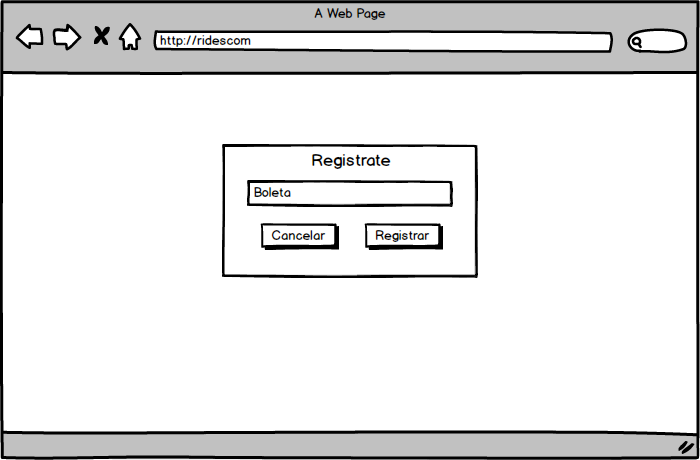
\includegraphics[width=10cm, height=6cm]{Imagenes/Disenos/VistasBorradas/p1_Registro.png}
		\caption{Registro para los alumnos.}
	\end{figure}
	
	\begin{figure}[hbt!]
		\centering
		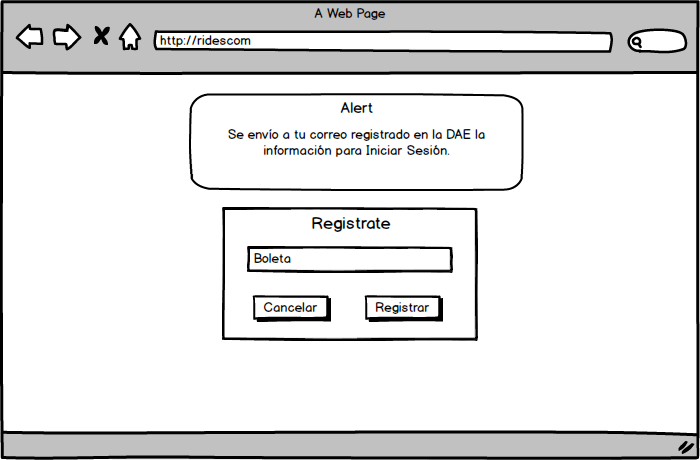
\includegraphics[width=10cm, height=6cm]{Imagenes/Disenos/VistasBorradas/ConfirmacionRegistro.png}
		\caption{Confirmación registro para los alumnos.}
	\end{figure}
	
	\begin{figure}[hbt!]
		\centering
		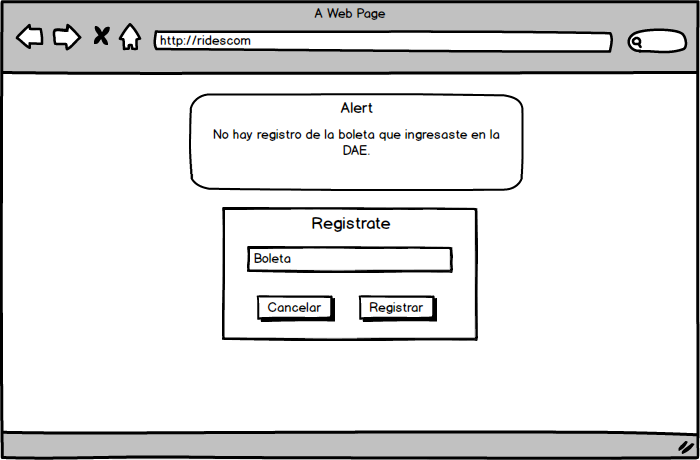
\includegraphics[width=10cm, height=6cm]{Imagenes/Disenos/VistasBorradas/p3RechazoRegistro.png}
		\caption{Rechazo registro para los alumnos.}
	\end{figure}

	\begin{figure}[hbt!]
		\centering
		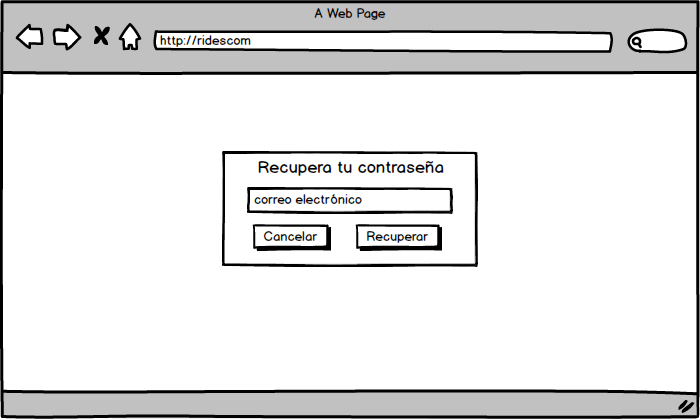
\includegraphics[width=10cm, height=6cm]{Imagenes/Disenos/VistasBorradas/p5Recuperarcontrasena.png}
		\caption{Recuperar contraseña para los alumnos.}
	\end{figure}

	\begin{figure}[hbt!]
		\centering
		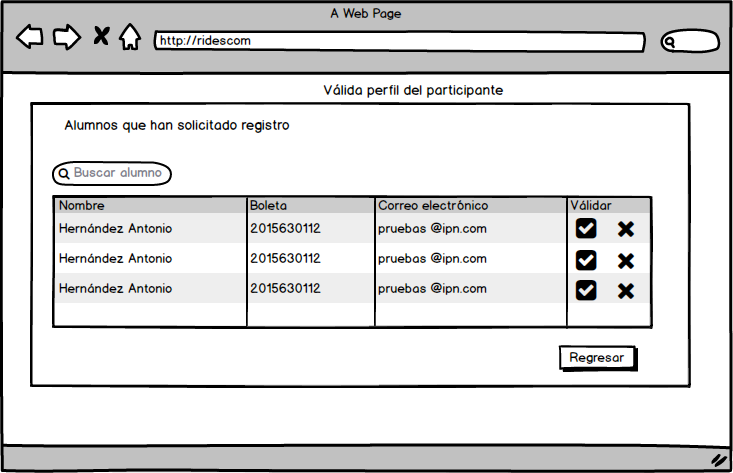
\includegraphics[width=10cm, height=6cm]{Imagenes/Disenos/VistasBorradas/p18ValidaPerfil.png}
		\caption{Validar perfil de los alumnos.}
	\end{figure}
	\pagebreak

	